\documentclass[pdflatex,sn-mathphys-num]{sn-jnl}

%%%% Standard Packages
\usepackage{graphicx}%
\usepackage{multirow}%
\usepackage{amsmath,amssymb,amsfonts}%
\usepackage{amsthm}%
\usepackage{mathrsfs}%
\usepackage[title]{appendix}%
\usepackage{xcolor}%
\usepackage{textcomp}%
\usepackage{manyfoot}%
\usepackage{booktabs}%
\usepackage{array}%
\usepackage{comment}
\usepackage{algorithm}%
\usepackage{algorithmicx}%
\usepackage{algpseudocode}%
\usepackage{listings}%
\usepackage{float}%

\newcommand{\placeholderfig}[2]{%
  \fbox{\parbox[c][#1][c]{0.92\textwidth}{\centering\sffamily\small
  [FIGURA PENDIENTE]\\[0.4em]#2}}%
}

\raggedbottom

\begin{document}

\title[How far do volcano-seismic classifiers generalize?]{How far do volcano-seismic classifiers generalize across volcanoes, stations and observatories?}
\author*[1,2]{\fnm{Sergio} \sur{Morales Méndez}}\email{s.morales01@ufromail.cl}
%\orcid{0000-0001-7848-8008}
\author[3]{\fnm{Andrés I.} \sur{Ávila}}\email{andres.avila@ufrontera.cl}

\author[4,5]{\fnm{Mailyn} \sur{Moreno Espino}}\email{mailymor@ucm.es}

\author[2]{\fnm{Oscar} \sur{Valderrama Cayumán}}\email{oscar.valderrama@sernageomin.cl}


\affil[1]{\orgdiv{Programa de Doctorado en Ingeniería}, \orgname{Universidad de La Frontera}, \orgaddress{\street{Francisco Salazar 01145}, \city{Temuco}, \postcode{4811230}, \country{Chile}}}

\affil[2]{\orgdiv{Observatorio Volcanológico de los Andes del Sur (OVDAS)}, \orgname{Servicio Nacional de Geología y Minería (SERNAGEOMIN)}, \orgaddress{\street{Rudecindo Ortega 03786}, \city{Temuco}, \postcode{4780000}, \country{Chile}}}

\affil[3]{\orgdiv{Departamento de Ingeniería Matemática}, \orgname{Universidad de La Frontera}, \orgaddress{\street{Francisco Salazar 01145}, \city{Temuco}, \postcode{4811230}, \country{Chile}}}

\affil[4]{\orgdiv{Facultad de Informática}, \orgname{Universidad Complutense de Madrid}, \orgaddress{\city{Madrid}, \country{España}}}

\affil[5]{\orgdiv{Instituto de Tecnología del Conocimiento}, \orgname{Universidad Complutense de Madrid}, \orgaddress{\city{Madrid}, \country{España}}}

\abstract{}
\keywords{}
\maketitle

%%===========================================================================%%
\section{Introduction}\label{sec:intro}

\section{Data}\label{sec:data}

\subsection{Volcanic systems and monitoring network}\label{subsec:area}

The study uses the seismic catalog of the Southern Andes Volcanological
Observatory (OVDAS), which monitors the active volcanoes of southern Chile
within the National Geology and Mining Service (SERNAGEOMIN)
\cite{amigo_volcano_2021} and keeps a continuous event catalog for the local
seismic network of each volcano. Five systems were selected for their large
event volumes, their joint coverage of the classes of interest and their
distinct volcanic environments.

These environments differ in the processes that drive their seismicity.
Villarrica is an open-conduit system with an active lava lake and
near-continuous long-period (LP) seismicity \cite{richardson_varying_2014}.
Nevados de Chill\'an has erupted since 2016, alternating effusive and
explosive phases \cite{cardona_volcanic_2021}. Copahue hosts persistent
hydrothermal circulation \cite{casas_single-station_2024}. Laguna del Maule
records a prolonged volcano-tectonic (VT) swarm linked to inflation of its
magmatic-hydrothermal system \cite{cardona_crustal_2018}. Hudson is a heavily
glaciated stratovolcano whose catalog combines brittle-fracture,
fluid-resonance and surface-process seismicity
\cite{agurto-detzel_seismicity_2014}.

The systems span about 1100~km of the Southern Volcanic Zone
(Figure~\ref{fig:map}), and each contributes the vertical channel of one
station, sampled at 100~Hz, over the interval covered by its analyzed events
(Table~\ref{tab:stations}). The records differ between systems in instrument
response, source--station distance, site conditions and event population.
Laguna del Maule starts in April 2021, after station NI2Z began operating on
30 March 2021. Copahue holds 99.1\% of its analyzed events between 2013 and
2016, and its station detects 979 events from 2017 to its last event in
August 2024. Hudson has 28 events in March 2013 and a record from June 2013
to January 2024 that includes months without events.

\begin{table}[h]
\caption{Station used at each volcanic system and the interval spanned by its
analyzed events (Table~\ref{tab:counts}).}\label{tab:stations}
\begin{tabular}{@{}lccc@{}}
\toprule
Volcanic system & Station & Crater distance (km) & Analyzed interval \\
\midrule
Laguna del Maule      & NI2Z & 7.4 & 2021-04--2024-12 \\
Nevados de Chill\'an  & FREZ & 1.6 & 2013-01--2024-12 \\
Copahue               & MAHZ & 3.7 & 2013-01--2024-08 \\
Villarrica            & VN2Z & 3.1 & 2013-01--2024-12 \\
Hudson                & HUDZ & 9.3 & 2013-03--2024-01 \\
\botrule
\end{tabular}
\end{table}

\begin{figure}[H]
\centering
\includegraphics[width=0.94\textwidth]{fig_map.pdf}
\caption{Location of the five volcanic systems and their stations, numbered
1--5 across panels. Left: regional view of the Southern Volcanic Zone, with a
globe inset. Right: shaded-relief local views of each crater (filled symbol)
and its station (open triangle, coded as in Table~\ref{tab:stations}); each
local panel has its own scale. Topography from Natural Earth and Terrarium
elevation tiles; coordinates in WGS84.}
\label{fig:map}
\end{figure}

\subsection{Nature of the catalog}\label{subsec:catalog}

Each catalog entry is an operational classification by an analyst, who
assigns the event class, the detecting station, an onset at that station and
a duration. The same class lasts differently at each system
(Table~\ref{tab:durations}): LP lasts 11.0~s at Copahue and 29.7~s at
Villarrica, and VT 8.0~s at Laguna del Maule and 17.9~s at Villarrica. A
non-positive duration appears in 654 entries at Nevados de Chill\'an, 514 at
Villarrica, 267 at Copahue, 22 at Hudson and none at Laguna del Maule, at most
0.24\% of the analyzed events of a system.

\begin{table}[h]
\caption{Median analyst-assigned duration in seconds within each volcanic
system and class, over the analyzed events with a positive duration; only
combinations with at least 50 events are shown.}\label{tab:durations}
\begin{tabular}{@{}lrrrrrr@{}}
\toprule
Volcano & LP & VT & HB & VLP & AV & TO \\
\midrule
Laguna del Maule      & 17.4 & 8.0  & --   & --   & --   & --   \\
Nevados de Chill\'an  & 28.0 & 13.0 & --   & 20.0 & 40.0 & 36.0 \\
Copahue               & 11.0 & 8.0  & 7.0  & 22.0 & --   & --   \\
Villarrica            & 29.7 & 17.9 & --   & --   & 27.0 & --   \\
Hudson                & 21.6 & 8.4  & 25.6 & --   & 20.0 & --   \\
\botrule
\end{tabular}
\end{table}

\subsection{Event classes}\label{subsec:classes}

The analysis uses six operational classes of the OVDAS database, based on the
classifications of \cite{lahr_earthquake_1994} and \cite{chouet_volcano_2003}:
LP (long-period), VT (volcano-tectonic), HB (hybrid), VLP (very-long-period,
coded LV), AV (avalanche and rockfall) and TO (tornillo), which account for
63--97\% of the catalog entries of each system between 2013 and 2024
(Table~\ref{tab:rawcounts}). All six are discrete events, which gives the
analysis a common unit of observation; the remaining codes describe sustained
tremor (TR), observational attributes, detections below the classification
threshold and further operational codes.

\begin{table}[h]
\caption{Catalogued entries between 2013 and 2024 at all stations of each
local network.}\label{tab:rawcounts}
\begin{tabular}{@{}lrrrr@{}}
\toprule
Volcano & Catalog total & Six retained classes & TR & Other codes \\
\midrule
Laguna del Maule
& 128{,}859
& 124{,}563 (96.7\%)
& 279 (0.2\%)
& 4{,}017 (3.1\%) \\
Nevados de Chill\'an
& 520{,}873
& 329{,}928 (63.3\%)
& 92{,}185 (17.7\%)
& 98{,}760 (19.0\%) \\
Copahue
& 160{,}526
& 150{,}405 (93.7\%)
& 5{,}643 (3.5\%)
& 4{,}478 (2.8\%) \\
Villarrica
& 1{,}198{,}979
& 1{,}008{,}464 (84.1\%)
& 112{,}301 (9.4\%)
& 78{,}214 (6.5\%) \\
Hudson
& 53{,}314
& 46{,}275 (86.8\%)
& 60 (0.1\%)
& 6{,}979 (13.1\%) \\
\botrule
\end{tabular}
\end{table}

Analysts assign the six classes from waveform morphology and spectral
content (Figure~\ref{fig:gallery}), so they are operational signal
categories, and the interpretations below are those commonly attached to
each label. LP events show emergent onsets and narrow-band low-frequency
energy, usually attributed to resonance in fluid-filled cracks
\cite{chouet_long-period_1996}. VT events show impulsive onsets and broadband
energy extending to higher frequencies, consistent with brittle rock failure.
HB events combine an impulsive onset with a low-frequency coda
\cite{white_volcano-tectonic_2016}. VLP events carry energy at lower
frequencies than LP and are linked to slow fluid transport or conduit
deformation \cite{almendros_identifying_2002}. AV events are emergent,
broadband and long surface signals \cite{heck_localization_2019}, and TO
events show slowly decaying, quasi-monochromatic codas
\cite{gomez_m_tornillo_1999}. The classes overlap in waveform and spectral
features, and HB in particular lies between LP and VT.

\begin{figure}[H]
\centering
\includegraphics[width=0.92\textwidth]{fig_gallery.pdf}
\caption{Representative waveform (left, first 10~s from the onset) and
amplitude spectrum of the same 10~s, normalized by its maximum (right), for
each retained class; each waveform panel gives the volcano and station of the
example.}
\label{fig:gallery}
\end{figure}

\subsection{Class composition}\label{subsec:composition}

The analyzed population is the part of the six-class catalog detected at the
station of Table~\ref{tab:stations} with a complete record around the event.
The two conditions retain 74--95\% of the six-class catalog, and the station
condition accounts for 78--95\% of the excluded entries
(Table~\ref{tab:filters}). Repeated entries with the same identifier and
time, 929 at Nevados de Chill\'an, 48 at Villarrica, 32 at Copahue and 3 at
Hudson, are counted once, and the five systems hold 34{,}140 to 959{,}236 distinct events each
(Table~\ref{tab:counts}).

\begin{table}[h]
\caption{Catalog entries remaining after each of the two conditions that
define the analyzed population, by system.}\label{tab:filters}
\begin{tabular}{@{}lrrrrr@{}}
\toprule
 & LdM & NdCh & Cop & Vil & Hud \\
\midrule
Six-class catalog        & 124{,}563 & 329{,}928 & 150{,}405 & 1{,}008{,}464 & 46{,}275 \\
Detected at the station  & 104{,}531 & 275{,}162 & 114{,}487 & 970{,}006 & 36{,}479 \\
\quad retained           & 83.9\% & 83.4\% & 76.1\% & 96.2\% & 78.8\% \\
With a complete record, distinct events & 103{,}476 & 268{,}011 & 112{,}547 & 959{,}236 & 34{,}140 \\
\quad retained           & 83.1\% & 81.2\% & 74.8\% & 95.1\% & 73.8\% \\
\botrule
\end{tabular}
\end{table}

\begin{table}[h]
\caption{Composition of the analyzed population by volcanic system and
class.}\label{tab:counts}
\begin{tabular}{@{}lrrrrrr@{}}
\toprule
Volcano & LP & VT & HB & VLP & AV & TO \\
\midrule
Laguna del Maule
& 446 & 102{,}962 & 22 & 0 & 46 & 0 \\
Nevados de Chill\'an
& 233{,}665 & 14{,}312 & 16 & 3{,}208 & 16{,}338 & 472 \\
Copahue
& 36{,}226 & 7{,}304 & 65{,}958 & 3{,}058 & 1 & 0 \\
Villarrica
& 952{,}458 & 314 & 1 & 23 & 6{,}440 & 0 \\
Hudson
& 10{,}940 & 15{,}035 & 483 & 0 & 7{,}682 & 0 \\
\botrule
\end{tabular}
\end{table}

Class composition varies strongly between systems. LP makes up 99.3\% of the
population at Villarrica and 87.2\% at Nevados de Chill\'an, VT 99.5\% at
Laguna del Maule and HB 58.6\% at Copahue, while Hudson has the most even
composition, with 44.0\% VT, 32.0\% LP, 22.5\% AV and 1.4\% HB. HB exceeds
50 events only at Copahue and Hudson, TO appears only at Nevados de
Chill\'an, and VLP concentrates at Nevados de Chill\'an and Copahue. These
proportions reflect the seismicity of each volcano together with network
sensitivity, station placement and labeling practice.

\subsection{Validation catalogs}\label{subsec:validation}

Four catalogs compiled by other agencies provide labeled records from other
volcanoes, networks and labeling practices (Table~\ref{tab:validation}), and
the study uses every class each catalog labels. LP and VT, present in all
four catalogs and at every OVDAS system, are the global labels; the classes
particular to one catalog or one observatory, HB, TO, VLP and AV at the OVDAS
systems and the other classes of Table~\ref{tab:validation}, are the local
labels. The events analyzed at each validation system are given in
Table~\ref{tab:valcounts} (Appendix~\ref{secA1}).

The Deception Island dataset
\cite{cortes_standardization_2019,cortes_vsr_2018} holds two deployments on this Antarctic volcano,
recorded at 50~Hz: a short-period sensor between the Argentinean and Spanish
bases in 1995 and a broadband station near the Spanish base in 2009. Its
label file gives the start and end of every event, often several per record,
as the volcano produces swarms. The study uses every LP, VT and NTR event,
the catalog's class for noise and tremor signals, and each deployment forms a
system of its own.

VCSEIS \cite{zhong_deep-learning-based_2024}, distributed in SeisBench format
\cite{woollam_seisbench_2022}, covers four regions catalogued by the Alaska
Volcano Observatory, the Hawaiian Volcano Observatory, the Northern
California Earthquake Data Center and the Pacific Northwest Seismic Network
(Cascade Range). Each trace is sampled at 100~Hz, carries P and S arrivals and
takes its class from the catalog field that separates long-period from local
events; an earthquake recorded at several stations appears once per station.
The study draws at random 500 LP and 500 VT traces per region and up to 500
traces of each further Alaska class: regional earthquakes, tremor, avalanches
and other events.

The VOISS-Net training set \cite{fee_generalized_2025} labels 120~s windows
of continuous data at volcanoes in Alaska, Hawai`i and Mexico, one label per
window and network. Its Earthquake and Long Period labels correspond to VT
and LP, and each volcano contributes one of them: VT at K\={\i}lauea,
Redoubt and Tanaga, LP at Veniaminof, Semisopochnoi and Pavlof. Its other
labels enter as local classes: harmonic, monochromatic and broadband tremor
at Pavlof and Semisopochnoi, harmonic tremor at Veniaminof and at
Popocat\'epetl, its only class, and explosions and noise at Pavlof and
Semisopochnoi. The study takes every labeled VT and LP window and up to 500
windows per volcano of each local class, drawn at random. The waveforms come
from the EarthScope data center, at the vertical channel of a reference
station per volcano or of the next station of a fixed list when it lacks the
window, from 60~s before to 120~s after each labeled window.

The Servicio Geol\'ogico Colombiano (SGC) provided 500 records per class,
labeled LP, VT, HB and tremor by its analysts; the letter R of the file
extension marks those from Nevado del Ruiz: 498 LP, 394 VT, 500 HB and 500
tremor, the last split into 250 of continuous tremor and 250 of tremor
pulses. Each record comes as one file with the stations available at the
time, sampled at a nominal 100~Hz, without catalog onset or duration. The SGC
designates Olleta as the reference station of the volcano and Bis as its
backup. The continuous-tremor files do not include Olleta, so continuous
tremor is recorded at Bis and tremor pulses at Olleta. At Olleta, 201 HB and
2 LP events come from OLLE, the single-component sensor of the older network,
taken as vertical, and the others from the vertical channel OLLZ.

\begin{table}[h]
\caption{Validation catalogs: the systems each contributes, its classes,
global (LP, VT) before the semicolon and local after it, its sampling rate,
and the reference times it supplies.}
\label{tab:validation}
\begin{tabular}{@{}>{\raggedright\arraybackslash}p{0.16\linewidth}
                >{\raggedright\arraybackslash}p{0.22\linewidth}
                >{\raggedright\arraybackslash}p{0.21\linewidth}
                >{\raggedright\arraybackslash}p{0.08\linewidth}
                >{\raggedright\arraybackslash}p{0.13\linewidth}@{}}
\toprule
Catalog & Systems & Classes & Rate (Hz) & Reference supplied \\
\midrule
Deception Island \cite{cortes_standardization_2019} & One volcano, two deployments (1995, 2009) & LP, VT; NTR & 50 & Segment start and end \\
VCSEIS \cite{zhong_deep-learning-based_2024} & Alaska, Cascade Range, Hawai`i, Northern California & LP, VT; regional, tremor, avalanche, other (Alaska) & 100 & P and S arrivals \\
VOISS-Net \cite{fee_generalized_2025} & K\={\i}lauea, Redoubt, Tanaga & VT & 50--100 & 120~s labeled window \\
 & Veniaminof, Semisopochnoi, Pavlof & LP; tremor & 50--100 & 120~s labeled window \\
 & Pavlof, Semisopochnoi & explosion, noise & 50 & 120~s labeled window \\
 & Popocat\'epetl & tremor & 40--100 & 120~s labeled window \\
SGC, Nevado del Ruiz & Olleta and Bis stations & LP, VT; HB, tremor & 100 & None \\
\botrule
\end{tabular}
\end{table}

The validation systems also differ in their recording conditions
(Table~\ref{tab:recording}). At five VOISS-Net volcanoes the reference
station records 93\% or more of the LP or VT windows; at Pavlof it records
57\%, and PVV and PN7A record the rest. The Tanaga station also lies 4.7~km
from neighboring Takawangha. The tremor of Popocat\'epetl is recorded at
four stations, and ZACA samples at
40~Hz in 243 of its 272 windows. Semisopochnoi, Tanaga, K\={\i}lauea and Deception Island stand on
oceanic islands, while the other validation volcanoes, like the five OVDAS
systems, stand on a continent.

\begin{table}[h]
\caption{Recording conditions of the validation systems. VOISS-Net: reference
station with its share of the LP or VT windows, its distance to the summit
\cite{gvp_votw} and its sampling rate; for Popocat\'epetl, the share of its
tremor windows at each station. VCSEIS: number of stations and median
epicentral distance, with the 10th and 90th percentiles, over the LP and VT
traces analyzed. Deception Island and Nevado del Ruiz: approximate distance
to the caldera center or to the Arenas crater, measured on the published maps
\cite{cortes_standardization_2019,castano_continuous_2020}.}\label{tab:recording}
\begin{tabular}{@{}>{\raggedright\arraybackslash}p{0.2\linewidth}
                >{\raggedright\arraybackslash}p{0.17\linewidth}
                >{\raggedright\arraybackslash}p{0.19\linewidth}
                >{\raggedright\arraybackslash}p{0.11\linewidth}
                >{\raggedright\arraybackslash}p{0.15\linewidth}@{}}
\toprule
System & Station & Distance (km) & Rate (Hz) & Setting \\
\midrule
\multicolumn{5}{@{}l}{\textit{VOISS-Net}} \\
K\={\i}lauea    & PUHI (93\%) & 5.4 & 100 & Island \\
Redoubt         & REF (99\%)  & 2.7 & 100 & Continental \\
Tanaga          & TASE (>99\%) & 9.3 & 50  & Island \\
Veniaminof      & VNSS (98\%) & 7.8 & 100 & Continental \\
Semisopochnoi   & CESW (93\%) & 3.6 & 50  & Island \\
Pavlof          & PV6A (57\%) & 11.2 & 50 & Continental \\
Popocat\'epetl  & ZACA (54\%), NEXP (24\%), HSHT (21\%) & -- & 40, 100 & Continental \\
\multicolumn{5}{@{}l}{\textit{VCSEIS}} \\
Alaska          & 161 stations & 8.6 (3.5--23.8)  & 100 & Mixed \\
Cascade Range   & 93 stations  & 15.0 (2.6--55.7) & 100 & Continental \\
Hawai`i         & 54 stations  & 4.5 (1.4--36.2)  & 100 & Island \\
N. California   & 97 stations  & 5.4 (1.8--20.9)  & 100 & Continental \\
\multicolumn{5}{@{}l}{\textit{Deception Island}} \\
1995            & Short-period sensor & $\approx$3 & 50 & Island \\
2009            & Broadband sensor    & $\approx$3 & 50 & Island \\
\multicolumn{5}{@{}l}{\textit{SGC, Nevado del Ruiz}} \\
Olleta          & OLLZ; OLLE (older network) & $\approx$2.4 & 100 & Continental \\
Bis             & BISZ, BIS1 & $\approx$1.1 & 100 & Continental \\
\botrule
\end{tabular}
\end{table}

%%===========================================================================%%
\section{Methodology}\label{sec:methods}

The pipeline turns each event into sixteen descriptors computed on two
windows of its waveform, a fixed-length window that opens at the onset and a
window that follows the event to the end of its coda. Every score is
measured within one system or one pair of systems, and every summary across
systems is built from those values.

\subsection{Station selection}\label{subsec:stationselection}

Each OVDAS system uses one station, the one that combines the largest number
of catalogued detections with uninterrupted operation
(Table~\ref{tab:stations}), which keeps a single instrument response and
source--station geometry within each class. Each validation catalog is
divided into systems following its own recording (Table~\ref{tab:recording}):
a VOISS-Net volcano gathers the windows of its reference station and of the
stations that replace it, a VCSEIS region the traces of all its stations, and
each SGC station and each Deception Island deployment forms a system of its
own.

\subsection{Fixed-length window}\label{subsec:conditioning}

The first window spans 10~s, 1{,}000 samples at 100~Hz, from the
analyst-assigned onset. It is cut from a segment padded from 7~s before the
onset to 13~s after it, linearly detrended and band-pass filtered between 0.5
and 10~Hz with a zero-phase fourth-order Butterworth filter; the 3~s margins
absorb the edge transient of the filter. The padded segment comes from one
gap-free trace of the selected station, so an event with a gap, an
interruption or a date before the station was installed falls outside the
analyzed population, the second condition of Table~\ref{tab:filters}, as
does an event whose filtered window has zero variance.

The signal-to-noise ratio of each event compares the signal window with a
2~s noise window, from 4 to 2~s before the onset, on the same filtered
segment:
\begin{equation}
\mathrm{SNR_{dB}} = 20\log_{10}\frac{\mathrm{RMS}(\text{signal window})}{\mathrm{RMS}(\text{noise window})}.
\end{equation}
The 2~s gap keeps an emergent arrival out of the noise window, and the band
of 0.5 to 10~Hz keeps out the secondary oceanic microseism, so the ratio
measures recording quality where the events radiate and, for VLP, the part of
the event within the band. The signal window is then z-scored to zero mean
and unit variance (Figure~\ref{fig:window}).

\begin{figure}[H]
\centering
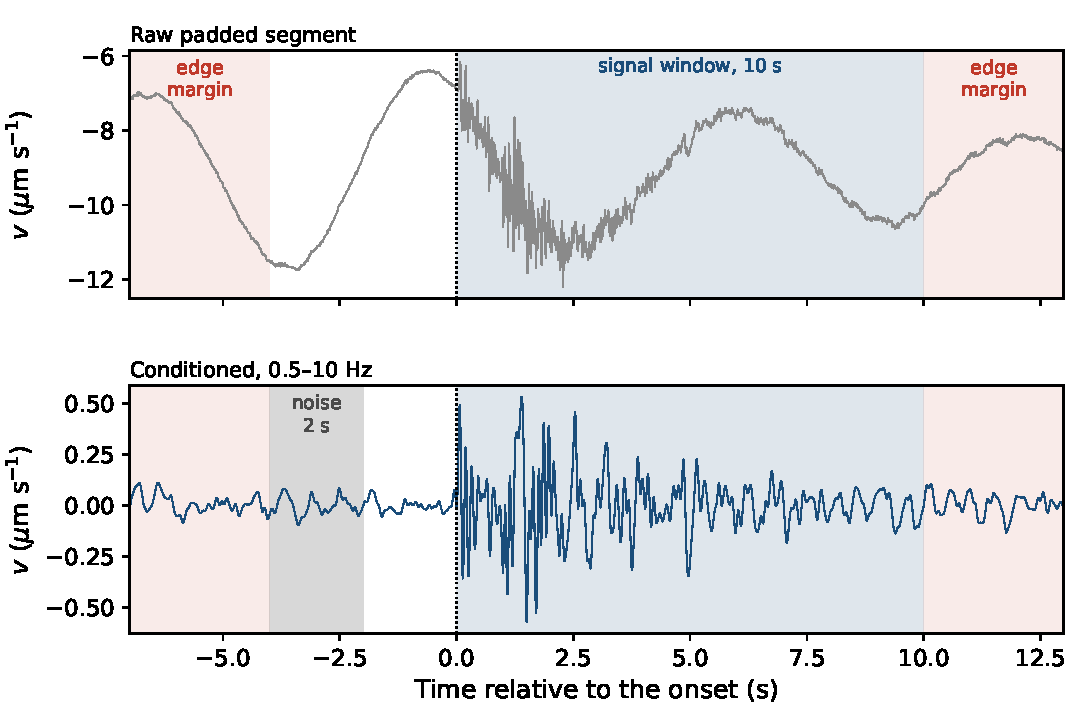
\includegraphics[width=0.94\textwidth]{fig_window.pdf}
\caption{Conditioning of the fixed-length window for a VT event at Hudson
(station HUDZ, signal-to-noise ratio 10.6~dB); dotted line: onset;
amplitudes in ground velocity. Top: raw padded segment,
from 7~s before to 13~s after the onset. Bottom: the same segment detrended
and band-passed between 0.5 and 10~Hz, with the discarded 3~s edge margins,
the 2~s noise window and the 10~s signal window shaded.}
\label{fig:window}
\end{figure}

\subsection{Coda-length window}\label{subsec:codawindow}

Many events outlast the fixed-length window (Table~\ref{tab:durations}),
which then measures their onset and early coda. A second window therefore
follows each event to the end of its coda, so that the two windows show
which properties of a class lie in its onset and which in its full coda.

The coda-length window opens at the onset and spans the duration of the
event, from 5~s, the shortest record that supports the recurrence
descriptors, to 100~s, after which a long coda is measured on its first
100~s, as in the full-duration window of \cite{morales_recurrence_2026}. The
duration is the analyst-assigned one at the OVDAS systems, and at the
validation systems the window runs to the end of the coda set by hand. Events shorter than 5~s,
including those with non-positive duration, keep only the fixed-length
window. The window is cut from a segment padded from 10~s before the onset to
3~s after the end of the window and conditioned as the fixed-length window, so the two
differ only in length; the lower corner of 0.5~Hz keeps both above the
secondary microseism, strong at the coastal and island validation stations.
Its noise window spans 5~s, from 7 to 2~s before the onset
(Figure~\ref{fig:codawindow}).

At four OVDAS systems the coda-length window is computed on a subsample of
the events lasting 5~s or more. Every class above the support criterion
enters in full up to $\rho$ times the size of the smallest of these classes,
and a larger class contributes that many events, taken at even steps through
the class in time order; $\rho$ is 10 at Laguna del Maule, Nevados de
Chill\'an and Copahue and 100 at Villarrica, whose smallest class is far
smaller than the others. Hudson enters in full. The analyses that compare the
two windows, the transferability ranking, the transferable plane and the
transfer matrices, use the events that hold both windows, so at these four
systems their fixed-length window covers the same subsample; the other
analyses take every event that holds the window they use.

\begin{figure}[H]
\centering
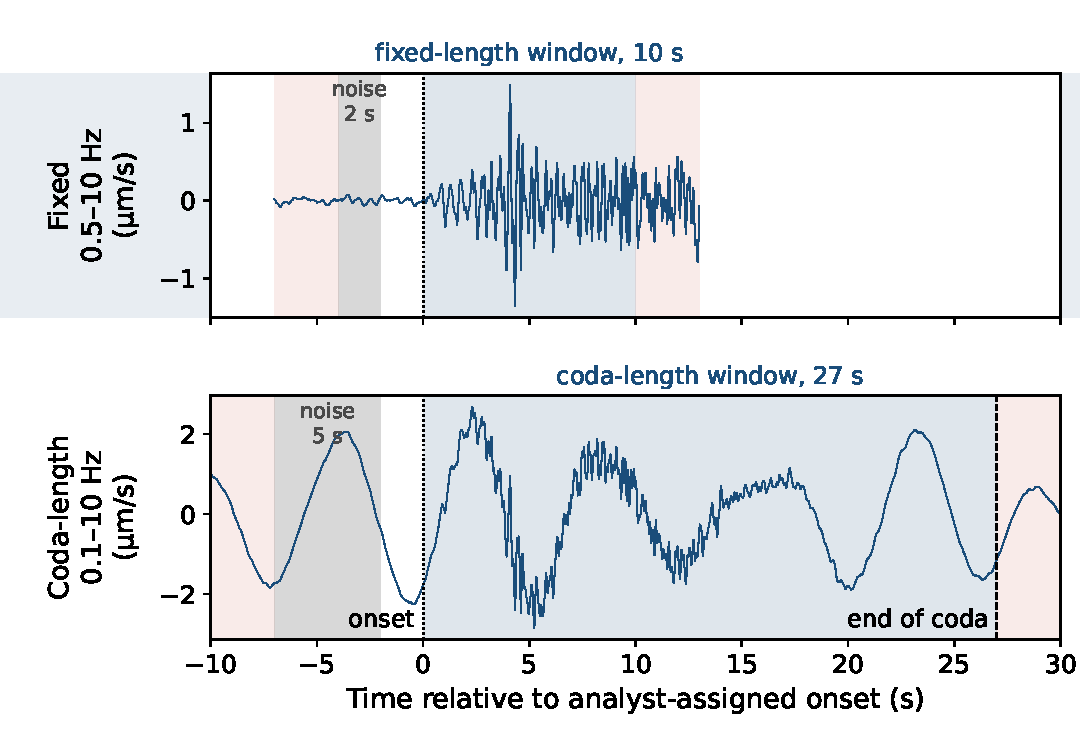
\includegraphics[width=0.94\textwidth]{fig_coda_window.pdf}
\caption{The two windows on one LP event at Hudson (station HUDZ,
analyst-assigned duration 27~s), conditioned between 0.5 and 10~Hz. Top:
fixed-length window with its 2~s noise window. Bottom: coda-length window, to
the end of the coda (dashed line), with its 5~s noise window. Dotted line:
onset; blue: signal window; grey: noise window; red: edge margins discarded
after filtering.}
\label{fig:codawindow}
\end{figure}

\subsection{Manual segmentation of the validation records}\label{subsec:manualcut}

The validation catalogs give labels but not the onset and end of the coda
that the windows need. One analyst therefore sets or confirms both for every
validation event, together with a pre-event noise window, under a single
protocol for the four catalogs (Figure~\ref{fig:manualcut}).

Each record is shown as its trace, band-passed between 0.5 and 10~Hz, and its
spectrogram up to 25~Hz, with the catalog reference and an automatic proposal that the analyst
accepts or corrects. The proposed onset is the catalog arrival or segment
start where one exists, and otherwise the first trigger of a recursive
STA/LTA detector (0.5 and 5~s windows, thresholds of 3 and 1, record
band-passed between 1 and 10~Hz) at least 5.5~s into the record, within the
labeled window or, for the SGC files, anywhere in the record. The proposed
end of the coda is the catalog segment end where one exists, and otherwise
the point where the envelope, smoothed over 1~s, falls below 1.2 times its
pre-event median for 2~s, with a proposed duration of at least 5~s; the
proposed noise window spans 12 to 2~s before the onset. The analyst places
the onset at the first arrival of the labeled event, the end of the coda
where the signal returns to the pre-event level, and the noise window right
before the onset, clear of other events where the record allows it. The
signal-to-noise ratio of both windows is measured as at the OVDAS systems,
from the onset set by the analyst; the manual noise window serves to choose
among copies of one event.

\begin{figure}[H]
\centering
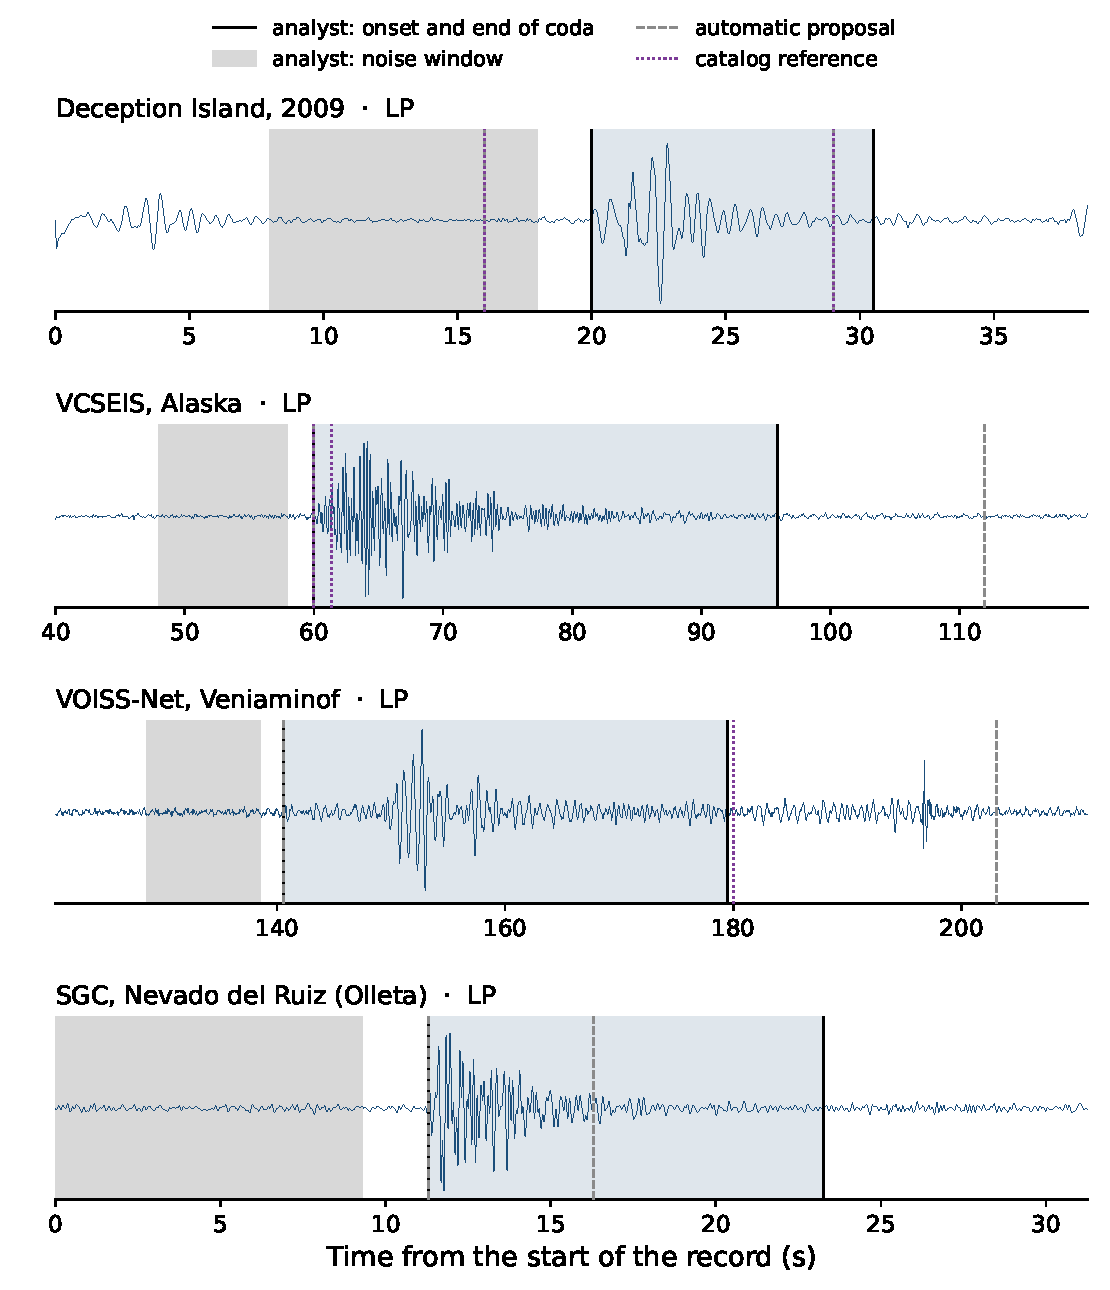
\includegraphics[width=0.94\textwidth]{fig_corte_manual.pdf}
\caption{Manual segmentation of one LP event from each validation catalog,
band-passed between 0.5 and 10~Hz and normalized. Dotted lines: reference
supplied by the catalog (none for the SGC); dashed lines: automatic proposal,
which at Deception Island coincides with the labeled segment; solid lines:
onset and end of the coda set by the analyst, with the signal window in blue
and the manual noise window in grey. The Nevado del Ruiz event is reviewed at
Olleta.}
\label{fig:manualcut}
\end{figure}

An event is kept when the analyst identifies the labeled event in the record
and its coda ends within the record, and it is discarded when no event is
visible in the catalog reference or when it lasts less than 5~s. The onset of
a kept event falls within the reference, from 2~s before its start, or, with
a flag, just outside it. Events marked as uncertain are kept, and an event
enters each window whose padded segment its record holds. At Nevado del Ruiz,
events are reviewed at Olleta and, when not visible there, at Bis, as the SGC
indicates, so Olleta and Bis differ both in the station and in the events
each records. VOISS-Net windows are reviewed in random order within each
volcano and class. An event the analyst relabels as a tornillo (TO) is
analyzed as LP, with a flag.

Each event is kept once. Of the copies of one earthquake at several VCSEIS
stations, which share a catalog source identifier, or of an event spanning
two consecutive VOISS-Net windows or SGC files, whose onsets lie less than
3~s apart, the copy with its onset inside the reference and the highest ratio
of the event to the manual noise window is kept. Records sampled at 50 or
40~Hz are resampled to 100~Hz by polyphase filtering before any other
filtering, and both windows and the sixteen descriptors are then computed
with the same code and parameters as at the OVDAS systems.

Explosions and the further VCSEIS classes, regional, tremor, avalanche and
other events, follow the same protocol, since they carry a catalog arrival or
a distinct first motion; of the regional and other events of Alaska, the
analyst reviews 26 and 228, respectively, and accepts the proposal, the catalog P arrival,
for the rest. The tremor of VOISS-Net and Nevado del Ruiz, noise and the
Deception Island NTR class are continuous signals with no onset, and they
enter through the fixed-length window alone, centered on the labeled span:
the 120~s window in VOISS-Net, the whole record at Nevado del Ruiz and the
labeled segment at Deception Island, extended where it is shorter than
10~s. Their window thus holds sustained signal rather than a first arrival, and
they carry no signal-to-noise ratio, since their noise window would fall
within the signal.

\subsection{Class support criterion}\label{subsec:classsupport}

A class enters the per-class analyses of a system when it holds at least 50
events there, a threshold that admits the local classes recorded at a single
volcano alongside the global ones. It is fixed before any analysis and
applies to every volcano-class combination of the OVDAS and validation
systems; a combination below it stays in the analyzed population.

\subsection{RQA and spectral feature extraction}\label{subsec:features}

Each window yields sixteen descriptors, thirteen from recurrence
quantification analysis (RQA) and three from the spectrum, computed on the
signal window of one event with the same parameters in both windows.

The recurrence descriptors $DET$, $L$, $L_{max}$, $DIV$, $L_{entr}$, $LAM$,
$TT$, $V_{max}$, $V_{entr}$, $W$, $W_{max}$, $W_{div}$ and $W_{entr}$
\cite{marwan_recurrence_2007} are those defined by
\cite{morales_recurrence_2026}, computed on the z-scored window with the
embedding that work selected on the OVDAS catalog by classifier performance:
dimension 2, delay of 3 samples and Theiler correction of 1, with diagonal,
vertical and white vertical lines counted from a length of 2 samples
(Figure~\ref{fig:rqa}). The radius $\varepsilon$ is set for each event from
the grid $\{0.1, 0.2, 0.4\}$ as the first with a recurrence rate ($RR$)
between 0.01 and 0.10, or otherwise the one with $RR$ closest to 0.03. $DIV$
and $W_{div}$ are the reciprocals of $L_{max}$ and $W_{max}$, so each pair
orders the events identically; they are left missing when that length is
zero, and all thirteen descriptors are left missing when every radius fails.
Where a later step needs complete values, a missing descriptor takes the
median of its system where each system is scaled on its own, and otherwise
the median of the training data for the logistic regression, while the
boosted trees take it as missing.

Three spectral descriptors complement this set. They come from the FFT of the
filtered window before z-scoring, over 1.0 to 8.0~Hz, where the filter passes
at least 89\% of the amplitude. $f_{\text{peak}}$ is the frequency of maximum
amplitude in that band, and $SR$ the ratio of mean to maximum amplitude
\cite{cui_subdivision_2021}, low for energy concentrated in a narrow band and
close to 1 for a flat spectrum. $FI$ compares two bands separated by a gap
\cite{cui_subdivision_2021,buurman_seismic_2010}:
\begin{equation}
\mathrm{FI} = \log_{10}\frac{\overline{A}(4.5\text{--}8.0~\mathrm{Hz})}{\overline{A}(1.0\text{--}2.5~\mathrm{Hz})},
\end{equation}
where $\overline{A}$ is the mean spectral amplitude of each band. One band
applies to every event, which keeps the descriptors comparable, so
$f_{\text{peak}}$ measures the dominant frequency of the classes that radiate
within it, LP and TO and most HB and AV events, and bounds it for the others:
it lies above the dominant frequency of VLP, which radiates mostly below
1~Hz, and at or below that of VT, which often exceeds 8~Hz
(Figure~\ref{fig:spectral}).

\begin{figure}[H]
\centering
\includegraphics[width=0.68\textwidth]{fig_rqa.pdf}
\caption{Recurrence plots of the six events of Figure~\ref{fig:gallery}, on
the z-scored signal window at the radius $\varepsilon$ selected for each
event, with its recurrence rate $RR$; axes run from the onset. The inset on
the VT panel enlarges 1~s from the middle of the window and marks the longest
diagonal line ($DET$, $L$, $L_{max}$, $DIV$, $L_{entr}$), vertical line
($LAM$, $TT$, $V_{max}$, $V_{entr}$) and white vertical line ($W$,
$W_{max}$, $W_{div}$, $W_{entr}$), offset by a few samples.}
\label{fig:rqa}
\end{figure}

\begin{figure}[H]
\centering
\includegraphics[width=0.98\textwidth]{fig_spectral.pdf}
\caption{The three spectral descriptors on the six events of
Figure~\ref{fig:gallery}, measured on the FFT of the conditioned window before
z-scoring. Shading: evaluation band, 1.0 to 8.0~Hz; dashed and dotted
horizontal lines: maximum and mean amplitude over that band, whose ratio is
$SR$; dashed vertical line: $f_{\text{peak}}$; coloured segments: mean
amplitude of the two bands entering $FI$. Values appear above each panel.}
\label{fig:spectral}
\end{figure}

\subsection{Descriptor transferability}\label{subsec:transferability}

A descriptor is transferable when it separates the global classes in the same
direction and with a similar strength at every system. Each descriptor is
scored at each system holding LP and VT above the support criterion by the
area under the ROC curve (AUC) of LP against VT, which needs no classifier
and no threshold, oriented by its median direction across systems, so a value
below 0.5 marks a reversal at that system. Descriptors are ranked by the
median oriented AUC across systems minus its interquartile range, which favors
descriptors that separate LP from VT at every system. The ranking is computed on each window over the events that
hold both windows, with up to 5{,}000 events per class of each system drawn
at random. The leading spectral and the leading recurrence descriptor of the
fixed-length window define the plane in which the global and local classes of
all systems are compared, in both windows. In that plane, LP and VT are drawn
as densities over all systems with equal weight for every system, and each
class of each system with at least 50 events by its median, with its
interquartile range for the local classes.

\subsection{Composition of the local classes}\label{subsec:heterogeneity}

A local class may gather events that the global classes would set apart, so
the composition of each local class is measured against LP and VT. For each
system, a logistic regression ($C = 1$), trained on the LP and VT events of
the other systems that hold both classes above the support criterion, leaving
out those of the same volcano and those sharing a station with it, with equal
total weight for each class of each training system, assigns every event of
the local class to LP, to VT or to neither. An event falls in neither when
the probability of its assigned class is below 0.7, or when its robust
Mahalanobis distance to that class, from a covariance fitted on up to 500
events of the class per training system, exceeds the 95th percentile of the
training events of the class, with every training system weighted equally.
The descriptors are scaled within each system with the median and
interquartile range of all its events, without labels, and each class of each
system enters with up to 3{,}000 events drawn at random. The analysis runs on
each window, with the continuous classes in the fixed-length window.

The same model scores the LP and VT events of the evaluated system as its
reference, and a local class is read only where that reference holds: each
global class of the system with at least 50 events is assigned correctly in
at least 80\% of its accepted events, with at most half of them rejected. A
composition is stable when its majority side, LP, VT or neither, persists
under two further scalings, one computed on the events left after capping
each class of the system at 3{,}000 and one shared by all systems, and the
reference of its system holds under all three. Gradient-boosted trees with
the first scaling check the side given by the logistic regression, and every
event keeps its catalog label.

\subsection{Classification and transfer design}\label{subsec:transfer}

Each system is first classified with all its classes above the support
criterion, global and local, by a logistic regression with a fixed
regularization strength and by gradient-boosted trees with a fixed
configuration, the same at every system, scored in each window by balanced
accuracy over five-fold cross-validation repeated five times on up to 300
events per class.

Generalization is measured by training a classifier on a single source
system and scoring it on another, and the scores of all source--target pairs
form a matrix for each window. The first matrix holds LP, VT and HB, the
classes that Nevado del Ruiz shares with the OVDAS taxonomy. Its sources are the systems with the three classes above the
support criterion, Copahue, Hudson and Nevado del Ruiz at Olleta, and Nevado
del Ruiz at Bis enters as a target scored on its LP and HB events. Its pairs
change the station within one volcano, from Olleta to Bis, together with the
events recorded; the volcano within one observatory, between Copahue and
Hudson; and both, between Nevado del Ruiz and the OVDAS systems, with HB
labeled by the analysts of two agencies.

The second matrix holds LP and VT. Its sources are the systems with both
classes above the support criterion, the five OVDAS systems, the four VCSEIS
regions and Nevado del Ruiz at Olleta, and its targets are every system with
LP or VT above that criterion, including those with a single class: the six
VOISS-Net volcanoes, Nevado del Ruiz at Bis and the 2009 Deception Island
deployment. Its pairs extend the sequence from volcanoes labeled by one
agency to volcanoes labeled by different agencies, the agency being the one
that draws the labels: OVDAS, the SGC, each observatory behind a VCSEIS
region, the VOISS-Net team and the Deception Island team. In both matrices
the diagonal, the source scored on its own events left out of each training
draw, is the reference, and the difference between a transfer score and the
diagonal score of its target is the transfer loss. Each step of the sequence
is summarized by the median over its pairs and over the medians of its
sources and of its targets.

Two classifiers are trained on each source. Gradient-boosted decision trees
\cite{chen_xgboost_2016} use the descriptors at their native scales, since a
tree ensemble is invariant to monotone rescaling, and an $L_2$-regularized
logistic regression uses them standardized with the mean and variance of its
training draw. A transfer loss shared by both models comes from the
descriptors and the records, and one seen only in the more flexible boosted
trees comes from what that model learned from its source.

A second scaling standardizes every system, source and target alike, with the
median and interquartile range of all its events, computed without labels,
and the logistic regression is then standardized with its training draw as
well. It removes a shift of the whole system in descriptor space, such as one from the site response or the source--station path, and keeps the
relations among its classes, so the difference between the two scalings
separates a transfer loss that a recalibration of the target recovers from
one that it does not. These statistics follow the class composition of a
system, so the second scaling is read only for targets that hold every class
of the matrix, and for a system dominated by one class its result reflects
that composition as well as the records.

Each training set holds 100 events per class drawn at random from the source,
a size that every class of every source exceeds in both windows, which keeps
sources of very different volume comparable and the class prior of the
source out of the decision. The draw is repeated 20 times, and each score is
reported as the mean and spread of the repetitions. The matrices use the
events that hold both windows, and at Copahue a fixed random set of
60{,}000 of them.

Hyperparameters are tuned on the source alone, on a separate draw of 100
events per class that may share events with the training draws and the
diagonal. For the boosted trees, a tree-structured
Parzen estimator \cite{akiba_optuna_2019} runs 200 trials that maximize the
balanced accuracy of stratified five-fold cross-validation on that draw, over
boosting rounds in $[200, 2000]$, maximum depth in $[3, 12]$, learning rate
in $[0.01, 0.3]$, row and column subsampling in $[0.5, 1.0]$, minimum child
weight in $[1, 50]$, and $L_1$ and $L_2$ regularization in $[10^{-8}, 10]$,
with the learning rate, child weight and both regularization terms sampled
log-uniformly. For the logistic regression, the same cross-validation
selects $C$ among 13 log-spaced values between $10^{-3}$ and $10^{3}$,
separately for each scaling. The configuration of a source stays fixed
across its 20 draws and all its targets.

Each target is scored by the recall of every class it holds and, when it
holds all the classes of the matrix, by their geometric mean,
\begin{equation}
G_m = \left( \prod_{c=1}^{C} \mathrm{recall}_c \right)^{1/C},
\end{equation}
which rewards recovering every class regardless of their proportion in the
target. Scores are computed on up to 5{,}000 events per class of the target,
drawn at random, and reported with the median and quartiles of their
signal-to-noise ratio. In the LP--VT matrix, the first draw of every source
also predicts each event of every target, and the recall of each class is
computed within each third of the target's signal-to-noise ratio, which
separates a loss that follows recording quality from one that follows the
source. Across the targets that hold LP and VT, the median score each target
receives is related by rank correlation to its median signal-to-noise ratio
and to its source--station distance, the station--crater distance at a
single-station target and the median epicentral distance at a VCSEIS region,
and island and continental targets are compared; across all targets, it is
related to the sampling rate. The permutation importance of each descriptor,
the drop in balanced accuracy averaged over three permutations, is computed
with the first scaling on every source--target pair, the diagonal included,
over the first three draws and up to 1{,}000 events of each target class
above the support criterion, and its median per descriptor is compared with
the ranking of Section~\ref{subsec:transferability} by rank correlation.

A detector tests whether a local class transfers like a global one. For each
local class present at two or more systems, a three-class model, the local
class against the LP and VT of the same system, is trained on up to 200
events per class of one system in five draws, on the fixed-length window with
up to 3{,}000 events per class and system. It is scored within its own system
by five-fold cross-validation and on every other system holding that class,
by the mean of the recall of the local class and the share of LP and VT
events not taken for it, a balanced accuracy. The model is a logistic
regression with balanced class weights and, as a contrast, gradient-boosted
trees with a fixed configuration, each with both scalings. The same procedure
with VT against LP is the reference of a global class, and the AUC of the
local class against LP and against VT in the target shows whether its
position between them is kept.

\subsection{Unsupervised grouping}\label{subsec:unsupervised}

The events of each system, global and local classes above the support
criterion together, up to 3{,}000 per class drawn at random, are grouped on
the fixed-length window with no label in the fit, by a full-covariance
Gaussian mixture on $FI$, $DET$ and $SR$, the three leading descriptors of
the transferability ranking, which uses the LP and VT labels of the same
systems, and, as a contrast, on all sixteen descriptors reduced by principal
components to 90\% of their variance. Each descriptor is standardized with
the median and interquartile range of all the events of its system; the
labels set only which classes enter and how many of their events.

The number of components is selected by stability. For each number from 2 to 8, or to 12 for the
joint grouping, mixtures are fitted on repeated 80\% draws, eight per system
on up to 800 events per class and twenty for the joint grouping. The retained
number is the largest one for which it and every smaller number reach a
median adjusted Rand index between draws of at least 0.8 and a 10th
percentile of at least 0.6; when no number does, two components are reported
as a grouping with no stable structure. The final partition is the medoid of
five fits on all events. Since the retained number can change with the
draws, the agreement with the labels and the search for recurrent groups
cover the whole range of component numbers.

The grouping runs within each system and on all systems together. The joint
grouping takes up to 300 events per class of each system, so that every
class of every system weighs the same, each standardized with the statistics
of its own system. Two variants of the joint grouping serve as contrast: one
computes the median and interquartile range of each system with equal weight
per class, and one, on $FI$, $DET$ and $SR$, takes up to 730 events per
system drawn at random regardless of class. The agreement with the catalog
labels, measured after the grouping and within each system, uses the
adjusted Rand index, the normalized mutual information and the share of each
class that falls in its majority group.

The joint grouping also tests for classes beyond the labels. A component is
a candidate for a further global class when LP and VT make up at most 30\%
of its events and it gathers at least 25\% of a local class, among classes
with at least 20 events, at three or more systems of at least two catalogs,
with at least two distinct local labels. A looser criterion keeps the same
recurrence but measures the share of local-class events only among the
members from systems that hold local classes, requires it to reach 0.70, and
compares it with the share those classes hold in the same systems.

\section{Results}\label{sec:results}

\subsection{Descriptor transferability}\label{subsec:res_transferability}

Five descriptors keep the direction of their contrast between LP and VT at
all ten systems that hold both classes, in both windows: $FI$, $SR$,
$f_{\text{peak}}$, $W$ and $W_{entr}$ (Table~\ref{tab:transferability};
Figure~\ref{fig:aucsystems} per system). $FI$ leads the ranking in both
windows, with a median oriented AUC of 0.93 and 0.94 and its lowest values,
0.73 and 0.76, in Alaska. In the fixed-length window $DET$, the
leading recurrence descriptor, and $SR$ follow with a median of 0.87; $DET$
reaches its lowest values at Nevado del Ruiz at Olleta (0.55) and Northern
California (0.59). In the coda-length window $SR$ rises to 0.89 and second
place, while $DET$ falls to 0.79 and reverses at Northern California.

The remaining recurrence descriptors reach median AUCs between 0.59 and 0.76,
and most of them reverse at one system, Northern California, except, in the
fixed-length window, $W_{max}$ and $W_{div}$, which reverse at Villarrica,
and $LAM$, which reverses at Olleta as well. $L_{max}$ and $DIV$,
like $W_{max}$ and $W_{div}$, share their AUC, so the sixteen descriptors
carry fourteen distinct contrasts, and $W_{max}$ and $W_{div}$ reverse their
direction between the two windows. The ranking thus sets apart a spectral
pair, $FI$ and $SR$, that carries LP and VT across systems in both windows,
and one recurrence descriptor, $DET$, that does so in the fixed-length window.
$FI$ and $DET$, the leading descriptor of each kind in that window, define
the common plane.

\begin{table}[h]
\caption{Transferability of the sixteen descriptors: median over the ten
systems with LP and VT of the AUC of LP against VT, oriented by its median
direction in the fixed-length window; its interquartile range (IQR); the
score, median minus IQR, that orders the table; and the number of systems
where the direction reverses.}
\label{tab:transferability}
\begin{tabular}{@{}llrrrrrrrr@{}}
\toprule
 & & \multicolumn{4}{c}{Fixed-length window} & \multicolumn{4}{c}{Coda-length window} \\
\cmidrule(lr){3-6}\cmidrule(l){7-10}
Descriptor & Direction & AUC & IQR & Score & Rev. & AUC & IQR & Score & Rev. \\
\midrule
$FI$ & LP$<$VT & 0.93 & 0.07 & 0.86 & 0 & 0.94 & 0.07 & 0.86 & 0 \\
$DET$ & LP$>$VT & 0.87 & 0.09 & 0.79 & 0 & 0.79 & 0.11 & 0.68 & 1 \\
$SR$ & LP$<$VT & 0.87 & 0.09 & 0.78 & 0 & 0.89 & 0.09 & 0.80 & 0 \\
$L_{entr}$ & LP$>$VT & 0.74 & 0.09 & 0.65 & 1 & 0.67 & 0.09 & 0.58 & 1 \\
$W_{max}$ & LP$<$VT & 0.72 & 0.08 & 0.64 & 1 & 0.68 & 0.17 & 0.51 & 0 \\
$W_{div}$ & LP$>$VT & 0.72 & 0.08 & 0.64 & 1 & 0.68 & 0.17 & 0.51 & 0 \\
$LAM$ & LP$>$VT & 0.76 & 0.14 & 0.62 & 2 & 0.68 & 0.13 & 0.55 & 1 \\
$L$ & LP$>$VT & 0.72 & 0.10 & 0.62 & 1 & 0.65 & 0.08 & 0.57 & 1 \\
$f_{\text{peak}}$ & LP$<$VT & 0.79 & 0.18 & 0.61 & 0 & 0.77 & 0.18 & 0.59 & 0 \\
$W$ & LP$>$VT & 0.70 & 0.13 & 0.57 & 0 & 0.71 & 0.10 & 0.60 & 0 \\
$W_{entr}$ & LP$>$VT & 0.68 & 0.12 & 0.56 & 0 & 0.74 & 0.13 & 0.61 & 0 \\
$V_{entr}$ & LP$>$VT & 0.66 & 0.17 & 0.49 & 1 & 0.60 & 0.05 & 0.55 & 1 \\
$TT$ & LP$>$VT & 0.65 & 0.17 & 0.48 & 1 & 0.60 & 0.04 & 0.56 & 1 \\
$V_{max}$ & LP$>$VT & 0.59 & 0.11 & 0.48 & 1 & 0.61 & 0.11 & 0.50 & 1 \\
$L_{max}$ & LP$>$VT & 0.60 & 0.14 & 0.46 & 1 & 0.62 & 0.09 & 0.53 & 1 \\
$DIV$ & LP$<$VT & 0.60 & 0.14 & 0.46 & 1 & 0.62 & 0.09 & 0.53 & 1 \\
\botrule
\end{tabular}
\end{table}

\begin{figure}[H]
\centering
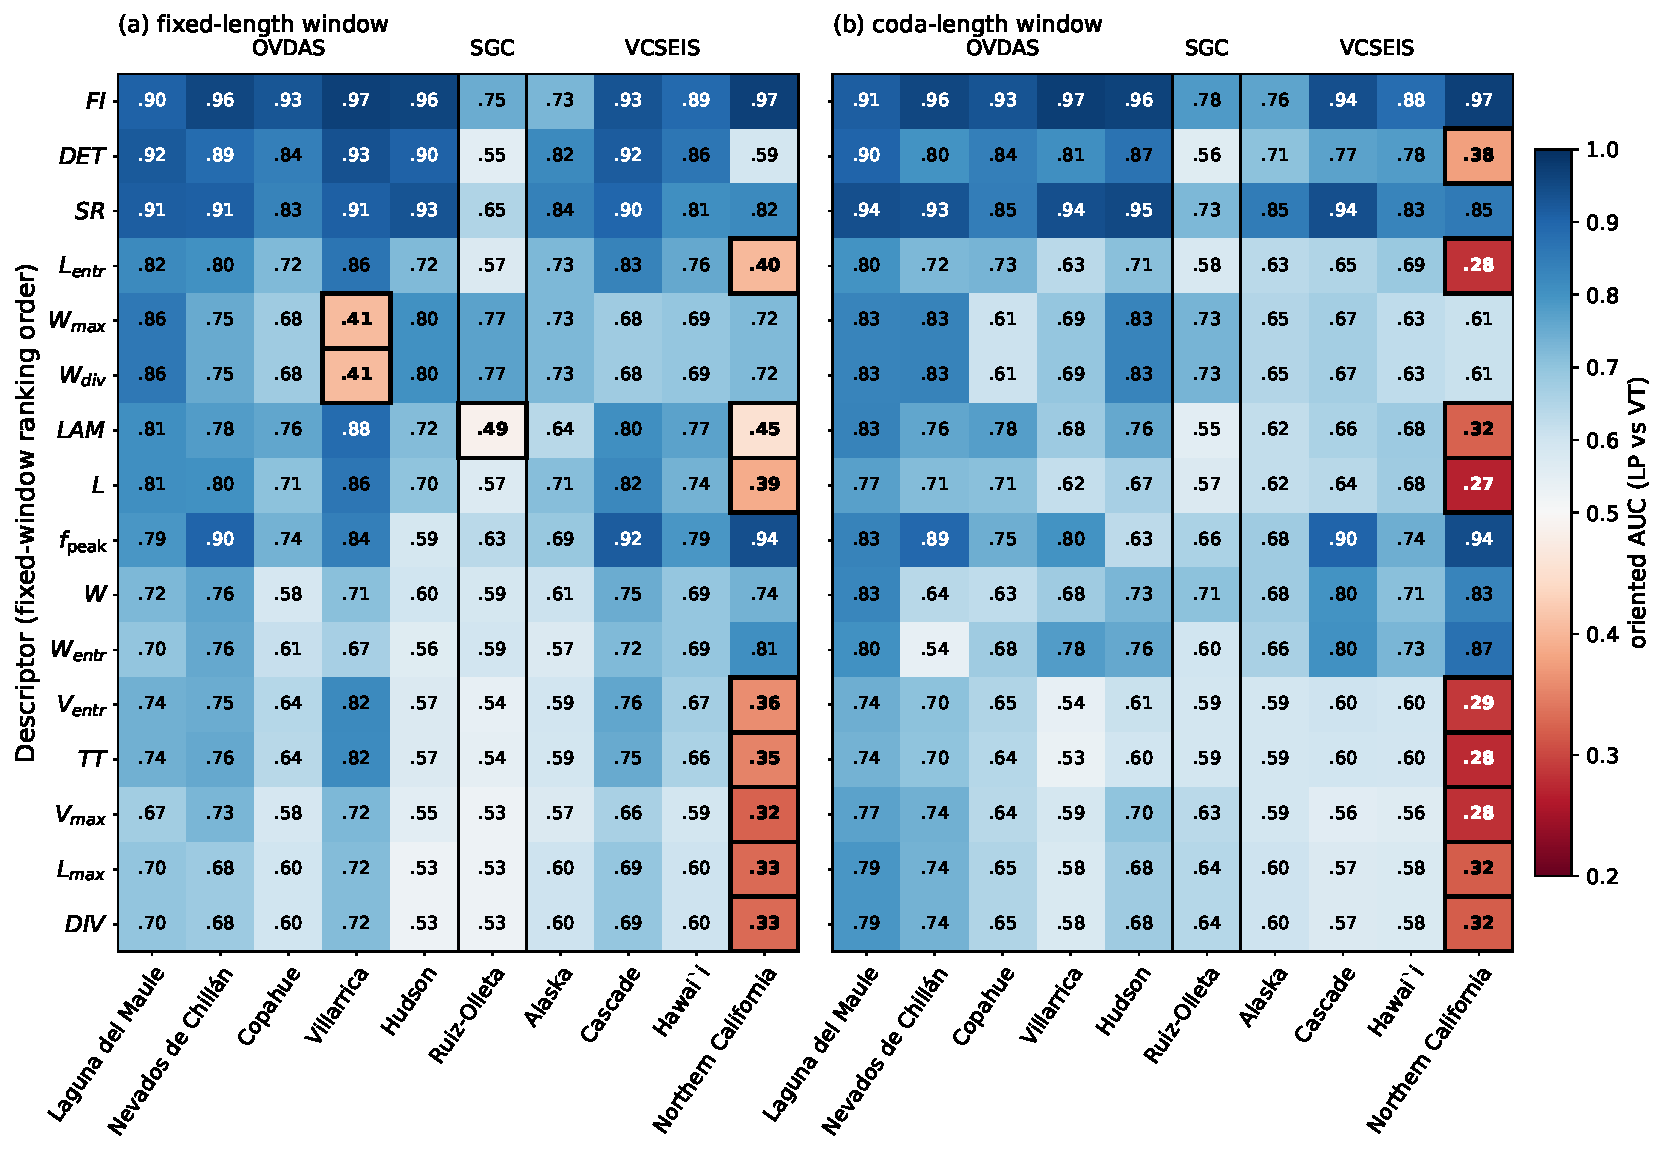
\includegraphics[width=0.98\textwidth]{fig_auc_por_sistema.pdf}
\caption{AUC of LP against VT per descriptor (rows, ordered as in
Table~\ref{tab:transferability}) and system (columns, grouped by agency),
oriented as in that table, for (a) the fixed-length and (b) the coda-length
window. Framed values below 0.5 mark a reversal at that system.}
\label{fig:aucsystems}
\end{figure}

\subsection{Global and local classes in the transferable plane}\label{subsec:res_plane}

In the plane of $FI$ and $DET$, LP gathers at low $FI$ and high $DET$, from
15 systems, and VT at higher $FI$ and lower $DET$, from 13
(Figure~\ref{fig:plane}). Every median of LP and VT lies within the 90\%
contour of its class, and most within its 50\% core. Outside the core lie,
in the fixed-length window, the LP medians of Copahue and Alaska and the VT
medians of Copahue, Hudson, Northern California and Redoubt, and in the
coda-length window the LP medians of Copahue, Laguna del Maule and Alaska and
the VT medians of Copahue, Hudson and Laguna del Maule. The LP medians of
Olleta and Bis lie within the LP contour and, in the fixed-length window,
inside the core of VT, next to the VT median of Olleta.

The local classes fall in places that depend on their catalog. In the
fixed-length window, the tremor types, noise and explosions of Pavlof and
Semisopochnoi, the harmonic tremor of Veniaminof and the NTR class of
Deception Island lie within the LP core, while the harmonic tremor of Popocat\'epetl lies between the two
clouds. The tremor of Nevado del Ruiz lies within the VT core at Olleta and
at the low-$DET$ edge of the VT cloud at Bis. HB lies between LP and VT at
Copahue, within the LP core at Hudson and within the VT core at Nevado del
Ruiz; AV within the VT core at Nevados de Chill\'an and Villarrica and
between the two clouds at Hudson; and the regional and other events of Alaska
within the VT core. The coda-length window keeps these positions, with HB of
Hudson leaving the VT contour and HB of Copahue the LP contour.

\begin{figure}[H]
\centering
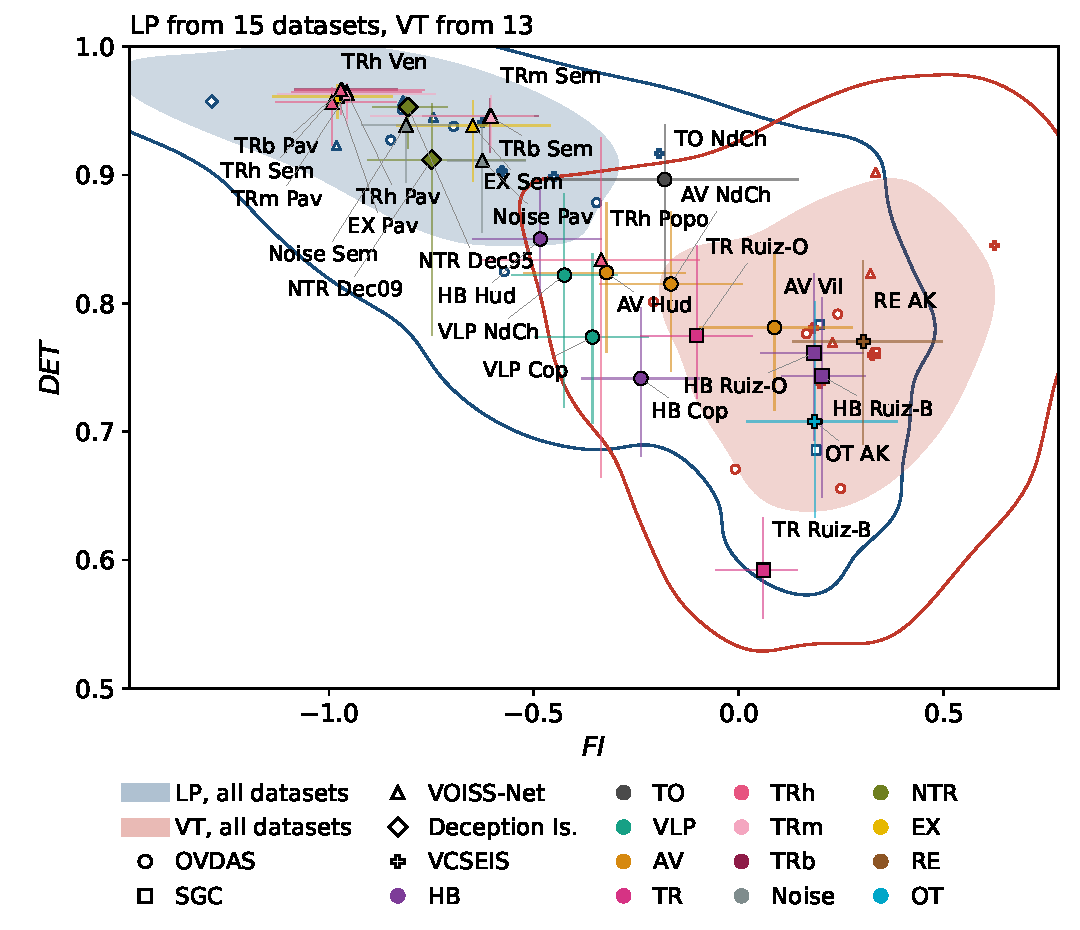
\includegraphics[width=0.8\textwidth]{fig_plano_transferible.pdf}
\caption{Global and local classes in the plane of $FI$ and $DET$, for the
fixed-length (top) and coda-length (bottom) windows. Shading encloses 50\%
and lines 90\% of the density of LP and of VT. Small open markers give the median of LP or VT at
each system, and large markers with bars the median and interquartile range
of each local class with at least 50 events. Marker shape gives the catalog
and color the class (TR: tremor of Nevado del Ruiz; TRh, TRm, TRb: harmonic,
monochromatic and broadband tremor of VOISS-Net; NTR: noise and tremor class
of Deception Island; EX: explosions; RE, OT: regional and other events of
Alaska). Popo: Popocat\'epetl; Dec95: Deception Island in 1995; other
abbreviations as in Figure~\ref{fig:matrices}. Tremor, noise and NTR have no
coda-length window.}
\label{fig:plane}
\end{figure}

Among the local classes, VLP keeps the most consistent position. At Copahue
and Nevados de Chill\'an, the only systems where it reaches the support
criterion, its median lies at $FI = -0.36$ and $DET = 0.77$ and at
$FI = -0.43$ and $DET = 0.82$, with $FI$ between the LP and VT of each system
and closer to LP, in both windows. Its logistic detector, with the source
scaling, reaches a balanced accuracy of 0.75 at Copahue and 0.89 at Nevados
de Chill\'an within each system, and keeps 0.73 from Copahue to Nevados de
Chill\'an and 0.66 in the opposite direction, while the same detector between
systems of one catalog reaches 0.53 for HB and 0.84 for VT against LP; the
second scaling and the boosted trees give 0.70 to 0.78 and 0.66 to 0.68 for
the two directions of VLP. This evidence rests on two systems of one agency,
and no validation catalog labels VLP, so its consistency holds within one
labeling practice, and its position reflects the part of its energy within
the bands the descriptors measure (Section~\ref{subsec:features}).

\subsection{Composition of the local classes}\label{subsec:res_heterogeneity}

The LP and VT reference holds at fewer systems than the local classes
require. In the fixed-length window, the complete reference holds only at
Copahue, Cascade Range, Hawai`i and Northern California, and the last three
hold no local class. The model trained on the other systems assigns less than
80\% of the accepted events correctly for LP at Villarrica (0.49), Nevados de
Chill\'an (0.51) and Nevado del Ruiz at Olleta (0.55), and for VT at Laguna
del Maule (0.23) and Alaska (0.72); at Hudson it assigns 0.796 of the
accepted VT events correctly and rejects 63\% of them. Among the systems with
a single global class, only the 2009 deployment of Deception Island holds its
reference. No local class of the fixed-length window has a stable
composition: where the reference fails the class cannot be read, and where it
holds, HB and VLP of Copahue and the NTR class of the 2009 deployment change
side between scalings.

In the coda-length window, the reference holds at Copahue, Hudson, Nevados
de Chill\'an and the four VCSEIS regions, and five local classes have a
stable composition (Table~\ref{tab:composition}); HB and AV of Hudson and VLP
of Copahue and Nevados de Chill\'an change side between scalings. HB of
Copahue and the regional and other events of Alaska fall mostly on the VT
side, the tornillos of Nevados de Chill\'an on the LP side, and AV of Nevados
de Chill\'an mostly on neither. In these five classes, 80\% to 100\% of the
events rejected as neither fall below the probability threshold, ambiguous
between LP and VT, rather than beyond the distance threshold. The two windows
enter with different scaling populations, the fixed-length one including the
continuous classes, so their difference in stability describes the two
readings together rather than the window alone.

\begin{table}[h]
\caption{Composition of the five local classes with a stable reading,
coda-length window: share of events assigned to LP, to VT and to neither.}
\label{tab:composition}
\begin{tabular}{@{}llrrrr@{}}
\toprule
System & Class & $n$ & LP & VT & Neither \\
\midrule
Copahue & HB & 3{,}000 & 0.14 & 0.54 & 0.32 \\
Nevados de Chill\'an & TO & 463 & 0.67 & 0.03 & 0.29 \\
Nevados de Chill\'an & AV & 3{,}000 & 0.17 & 0.29 & 0.54 \\
Alaska & Other & 340 & 0.11 & 0.59 & 0.30 \\
Alaska & Regional & 162 & 0.09 & 0.57 & 0.35 \\
\botrule
\end{tabular}
\end{table}

\subsection{Transfer across systems}\label{subsec:res_transfer}

With all their classes, the descriptors separate the taxonomy of each system
to a degree that falls with the number and the overlap of its classes
(Figure~\ref{fig:confusion}, Appendix~\ref{secA1}). With the boosted trees in
the fixed-length window, the balanced accuracy is 0.97 at Laguna del Maule,
0.83 to 0.94 at the three VCSEIS regions with two classes, 0.92 at Deception
Island in 2009 and 0.80 at Veniaminof, also with two; 0.81 at Villarrica with
three and 0.75 at Nevados de Chill\'an with five; 0.62 to 0.67 at Copahue,
Hudson and both stations of Nevado del Ruiz, which hold HB; 0.53 in Alaska
with four; and 0.45 and 0.51 at Pavlof and Semisopochnoi with six, against
chance levels of 0.17 to 0.50. VLP and TO at Nevados de Chill\'an reach
recalls of 0.80 and 0.79, while HB, AV, explosions, the regional events of
Alaska and the three tremor types of VOISS-Net among themselves stay between
0.18 and 0.74, with errors that follow the overlaps of each system, as at
Nevado del Ruiz, where 0.36 of the LP events of Olleta are taken for HB and
0.67 of the HB events of Bis for LP. Tremor at Nevado del Ruiz, noise at
Pavlof and Semisopochnoi and the NTR class of Deception Island reach recalls
of 0.83 to 0.95; these continuous classes enter with a window centered on the labeled span rather than one starting at an onset
(Section~\ref{subsec:manualcut}), so their recall reflects that window
together with their content.

The diagonal of the LP--VT transfer matrix reaches a median $G_m$ of 0.90 to 0.91 in both windows, lowest at
Nevado del Ruiz at Olleta, Hawai`i and Alaska (0.77 to 0.84) and highest at
Laguna del Maule (0.95 to 0.96; Figure~\ref{fig:matrices}). Here and below, a range spans the two classifiers
and, where stated, the two windows. The standard deviation of $G_m$ over the
20 draws has a median of 0.02 to 0.03 per pair and reaches at most 0.12.

\begin{figure}[H]
\centering
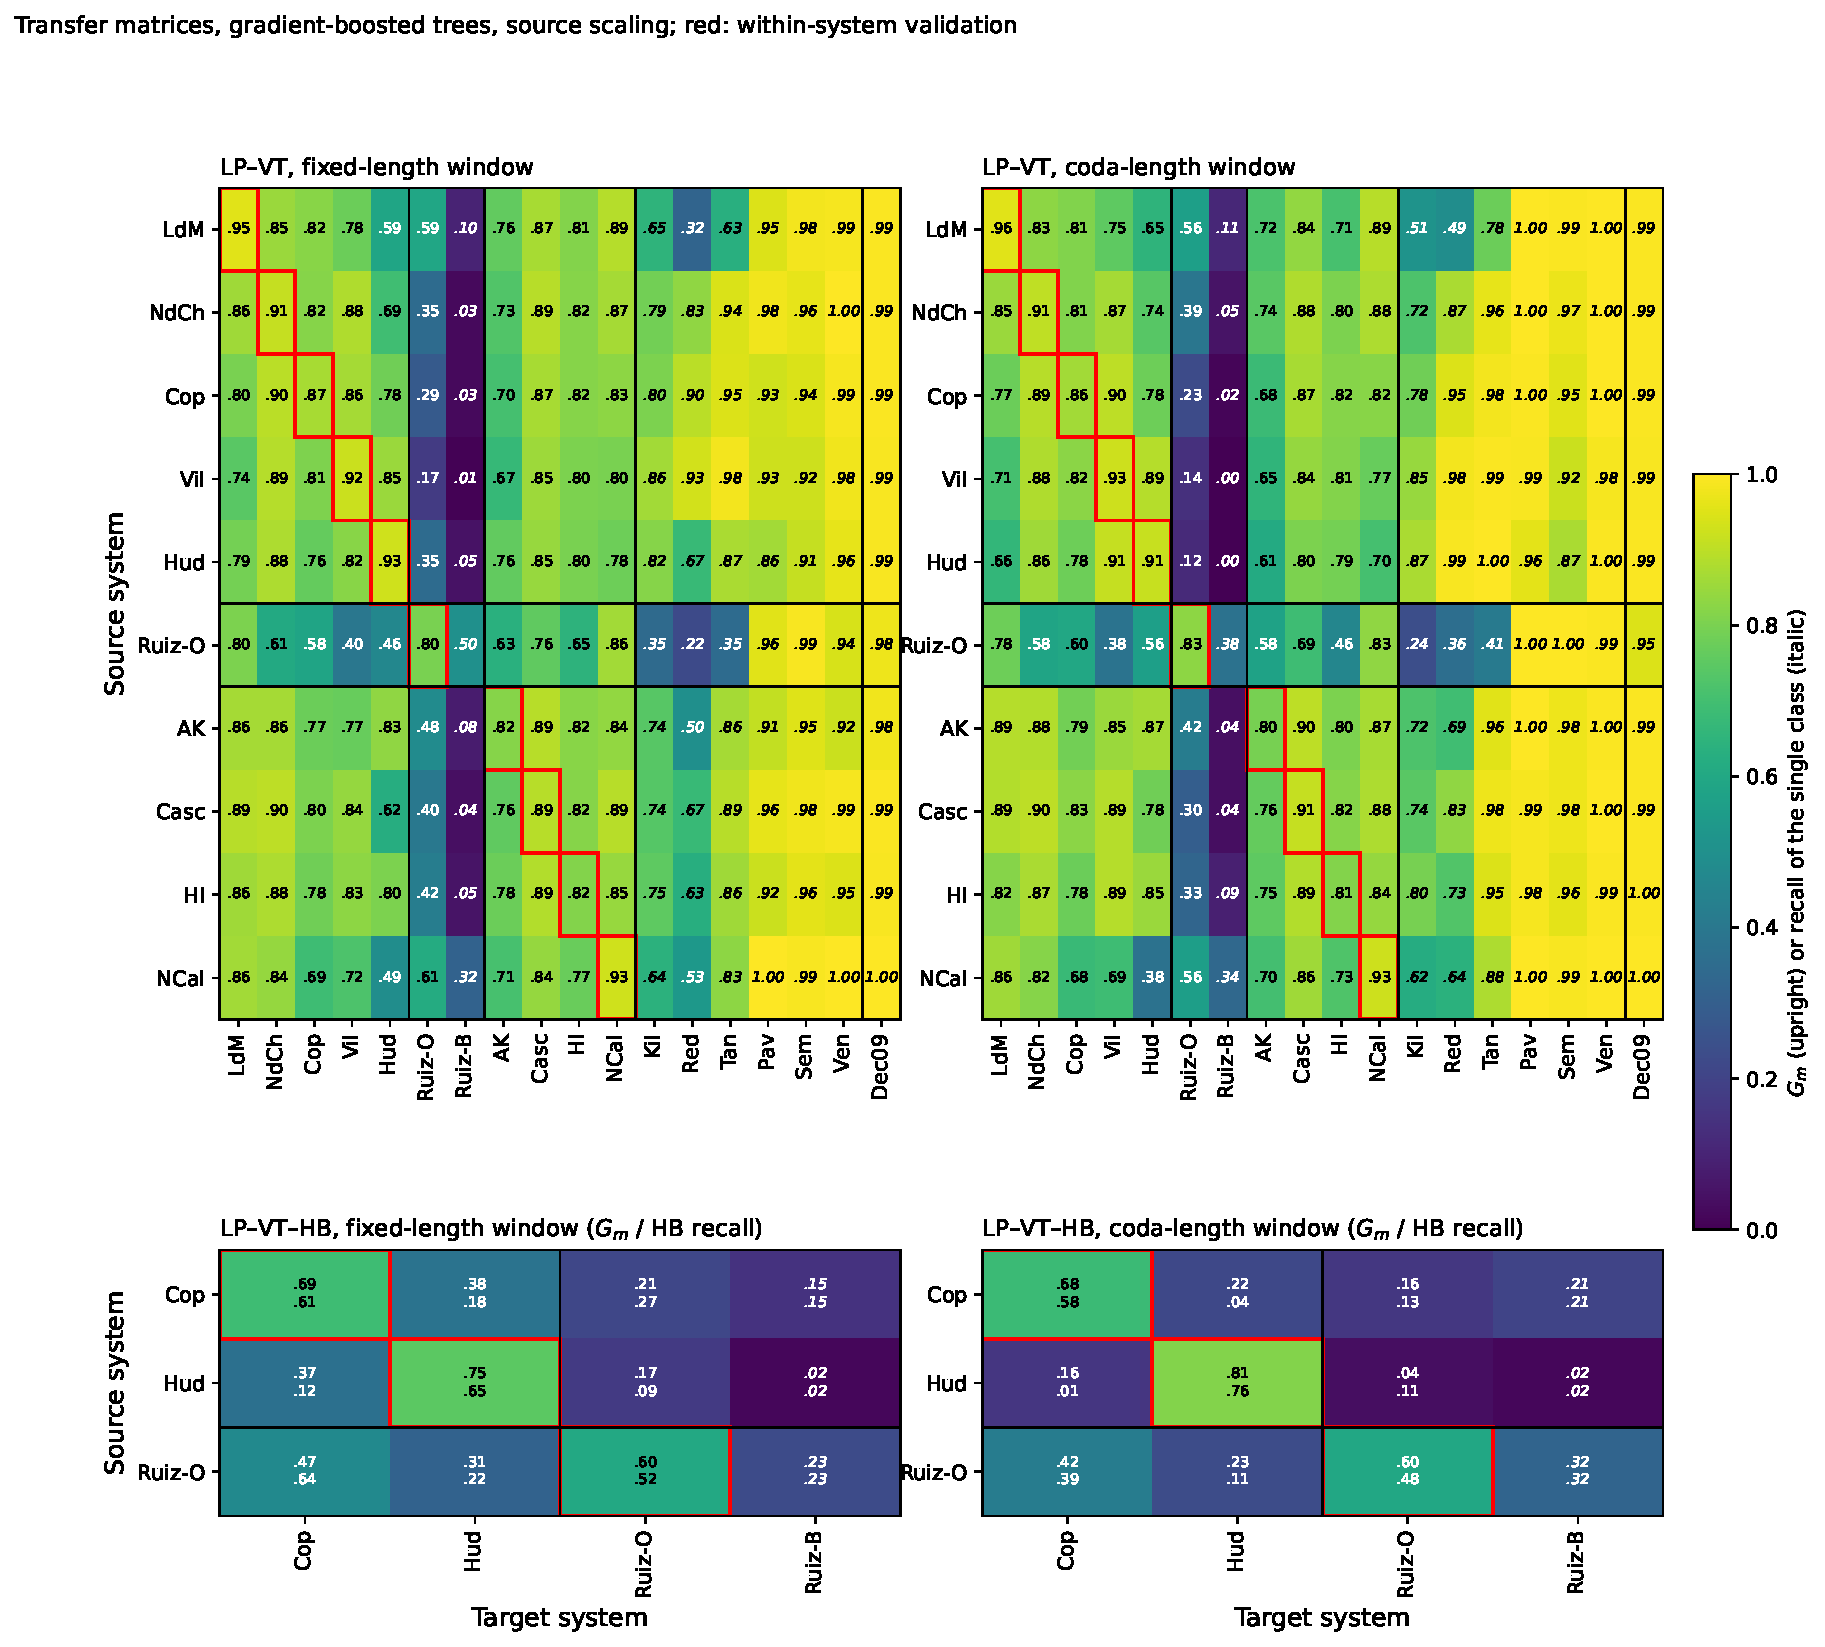
\includegraphics[width=0.98\textwidth]{fig_matrices_transferencia.pdf}
\caption{Transfer matrices of the gradient-boosted trees with the source
scaling, mean of 20 draws, for the fixed-length (left) and coda-length
(right) windows; rows give the source and columns the target, grouped by
catalog. Top: LP--VT, with $G_m$ when the target holds LP and VT and, in
italics, the recall of its single class otherwise. Bottom: LP--VT--HB, with
$G_m$ above and the recall of HB below; at Nevado del Ruiz at Bis, which lacks
VT, both lines give the recall of HB, in italics. Red frames mark the
within-system validation. LdM, NdCh, Cop, Vil, Hud: Laguna del Maule,
Nevados de Chill\'an, Copahue, Villarrica, Hudson; Ruiz-O, Ruiz-B: Nevado del
Ruiz at Olleta and at Bis; AK, Casc, HI, NCal: Alaska, Cascade Range,
Hawai`i, Northern California; Kil, Red, Tan, Pav, Sem, Ven: K\={\i}lauea,
Redoubt, Tanaga, Pavlof, Semisopochnoi, Veniaminof; Dec09: Deception Island
in 2009.}
\label{fig:matrices}
\end{figure}

LP and VT transfer with a moderate loss, and a change of labeling agency
lowers the score no more than a change of volcano within one agency. In the
fixed-length window, moving to another volcano of the same agency, here between OVDAS systems, lowers the median $G_m$ per pair to 0.85
with the logistic regression and 0.82 with the boosted trees, and moving to
another agency to 0.82 and 0.80; the median transfer loss is 0.07 with the
logistic regression and 0.09 with the boosted trees in both steps. With the
medians taken by source or by target, both steps lie between 0.79 and 0.84
and change order. The coda-length window gives 0.78 to 0.83 outside the
diagonal, and the two classifiers differ by at most 0.05 at every step. With
the second scaling, the step within one agency falls to 0.71 to 0.73 in the
fixed-length window and 0.64 to 0.69 in the coda-length window, and the step
between agencies to 0.77 to 0.79 and 0.76; that scaling follows the class
composition of each system, which differs most among the OVDAS systems
(Table~\ref{tab:counts}).

Most single-class targets keep their class: over all sources, the
median recall of LP at the VOISS-Net volcanoes and at the 2009 Deception
Island deployment is 0.92 to 1.00, and that of VT at Tanaga, K\={\i}lauea and
Redoubt 0.87 to 0.96, 0.73 to 0.76 and 0.65 to 0.78, over both windows. This
recall measures how much of the class a source recovers, not its separation
from the class the target lacks. The four targets sampled at 50~Hz all hold
a single class, so over the eighteen targets the score falls with the
sampling rate (Spearman $\rho = -0.62$) together with the change from two
classes to one. Nevado del Ruiz at Bis is the exception: the median recall of
its LP over all sources is 0.03 to 0.06 in both windows, 0.38 to 0.50 when the
source is Olleta, on the same volcano but with the events not visible there,
and lower from every other system.

HB loses most of its recall between
systems: from 0.57 to 0.61 within its system in the fixed-length
window, it falls to 0.15 to 0.16 between Copahue and Hudson, to 0.19 to 0.20
between agencies and to 0.23 to 0.35 from Olleta to Bis. The $G_m$ of the
three classes is 0.68 to 0.69 within each system, 0.36 to 0.37 between
Copahue and Hudson and 0.22 to 0.26 between agencies. The step between
Copahue and Hudson rests on two pairs, and HB makes up 58.6\% of the analyzed
population at Copahue and 1.4\% at Hudson. When the target is Nevado del
Ruiz, its LP collapses as well, to recalls of 0.002 to 0.077 from Copahue and
Hudson. The second scaling recovers part of HB, to recalls of 0.31 to 0.40
and a $G_m$ of 0.45 to 0.49, without approaching the diagonal.

The detectors set each local class beside the VT against LP reference of the
same pairs. Over the four pairs between Copahue or Hudson and Olleta, the
logistic detector with the source scaling reaches a balanced accuracy of
0.44 to 0.59 for HB and 0.54 to 0.59 for the reference, so at this step HB
and the global classes fail together; with the second scaling the reference
rises to 0.64 to 0.82, while HB stays at 0.53 to 0.58. Between Copahue and
Hudson, HB reaches 0.43 to 0.52 against 0.77 for the reference with the
source scaling, and 0.53 to 0.57 against 0.84 to 0.87 with the second
scaling. HB therefore falls below the global classes within one agency and
wherever each system is scaled on its own events. Tremor has no matched
reference, since the VOISS-Net volcanoes hold no pair of LP and VT; its
logistic detector reaches 0.77 to 0.78 within each system, 0.60 to 0.63
between systems of one catalog and 0.49 between VOISS-Net and Nevado del
Ruiz, where the AUC of tremor against LP is about 0.48. With boosted trees,
these detectors reach 0.51 for HB and 0.48 for tremor between catalogs.

The transferred models rely on the transferable descriptors
(Figure~\ref{fig:importance}, Appendix~\ref{secA1}). In the LP--VT matrix
with the fixed-length window, permuting $FI$ costs the boosted trees the most
balanced accuracy from seven of the ten sources, 8 to 31 percentage points as
a median over targets, while $DET$ leads from Alaska and Hawai`i and
$f_{\text{peak}}$, by one point, from the Cascade Range; within each system
the median importance is 16 points for $FI$, 8 for $DET$ and 1 for $SR$. In
the coda-length window $FI$ leads from eight sources, and $SR$ takes the
weight of the recurrence descriptors and leads from Alaska and the Cascade
Range. In the LP--VT--HB
matrix, $FI$ and $DET$ carry 13 and 10 points within each system, while in
transfer no descriptor reaches 5 points from any source. Beyond $FI$, $DET$,
$SR$ and $f_{\text{peak}}$, no descriptor reaches 4 points from any source,
so the agreement with the ranking of Table~\ref{tab:transferability} rests on
its first places: $FI$, $DET$ and $SR$ are the three most important
descriptors with both classifiers in the fixed-length window, within each
system and in transfer, and in the coda-length window $FI$ leads, followed by
$DET$ with the logistic regression and by $SR$ with the boosted trees. The
rank correlation over the sixteen descriptors, 0.72 to 0.92 in the
fixed-length window and 0.46 to 0.70 in the coda-length window, also reflects
the order of the near-zero importances.

Recording quality shapes part of the loss within the targets. With the
boosted trees in the fixed-length window, from the lowest to the highest
third of signal-to-noise ratio the recall rises by more than 0.03 at 13 of
the 28 combinations of target and class, stays within 0.03 at 11 and falls at
4; the LP of Bis stays at 0.06 to 0.10. Across the ten targets with LP and VT, the
median score correlates weakly with the median signal-to-noise ratio of the
target, with a Spearman $\rho$ of 0.26 to 0.47 over the two windows and
classifiers ($p \geq 0.17$), and with the source--station distance, with
$|\rho| \leq 0.26$. Hawai`i, the only island target with both classes,
differs from the median of the continental targets by at most 0.03.

\subsection{Unsupervised grouping}\label{subsec:res_unsupervised}

Without labels in the fit, the descriptors group the events of a system only
partly by class (Figure~\ref{fig:grouping}a). Within each system, the mixture
on $FI$, $DET$ and $SR$ reaches a median adjusted Rand index of 0.22 with the
catalog labels, from 0.02 to 0.63. The highest values come from systems with
two or three classes, Cascade Range (0.63), Hawai`i (0.42), Northern
California (0.38), Villarrica (0.33) and the 2009 Deception Island deployment
(0.32), and at the seven systems with four to six classes the index stays at
or below 0.22; with all sixteen descriptors the median falls to 0.11. Grouping all
systems together gives a median index per system of 0.10 to 0.14 with $FI$,
$DET$ and $SR$ and 0.03 to 0.06 with all sixteen, over the variants, whose
stable number of components varies between 2 and 5
(Figure~\ref{fig:grouping}c).

At five components, the largest stable number of the joint grouping, reached on $FI$, $DET$ and $SR$ with all events, it returns a
low-frequency, highly deterministic group (Figure~\ref{fig:grouping}b, G4).
It gathers more than half of the tremor types and explosions of Pavlof, of
the harmonic tremor of Semisopochnoi, Popocat\'epetl and Veniaminof, of the
noise of Semisopochnoi, of the 1995 NTR class of Deception Island, of HB of
Hudson and of the tremor of Nevado del Ruiz at Olleta; about half of VLP of
Copahue, AV of Hudson and the 2009 NTR class; and most LP events of the four
VCSEIS regions, of the 2009 Deception Island deployment and of the OVDAS
systems other than Laguna del Maule, so that LP and VT make up 49\% of its
events. No group of any variant or number of components, from 2 to 12,
recurs at three or more systems of two or more catalogs with at most 30\% of
LP and VT. Nine groups meet the looser criterion, eight from the sixteen
descriptors and one from $FI$, $DET$ and $SR$, all at more components than
the stable number of their variant, and their local share, at most 0.73,
exceeds the base of 0.62 by a factor of at most 1.18; one of them spans ten
systems, five catalogs and thirteen local labels with 42\% of LP and VT. The
local classes thus fall within the regions of LP and VT, mostly that of LP,
rather than forming a group of their own.

\begin{figure}[H]
\centering
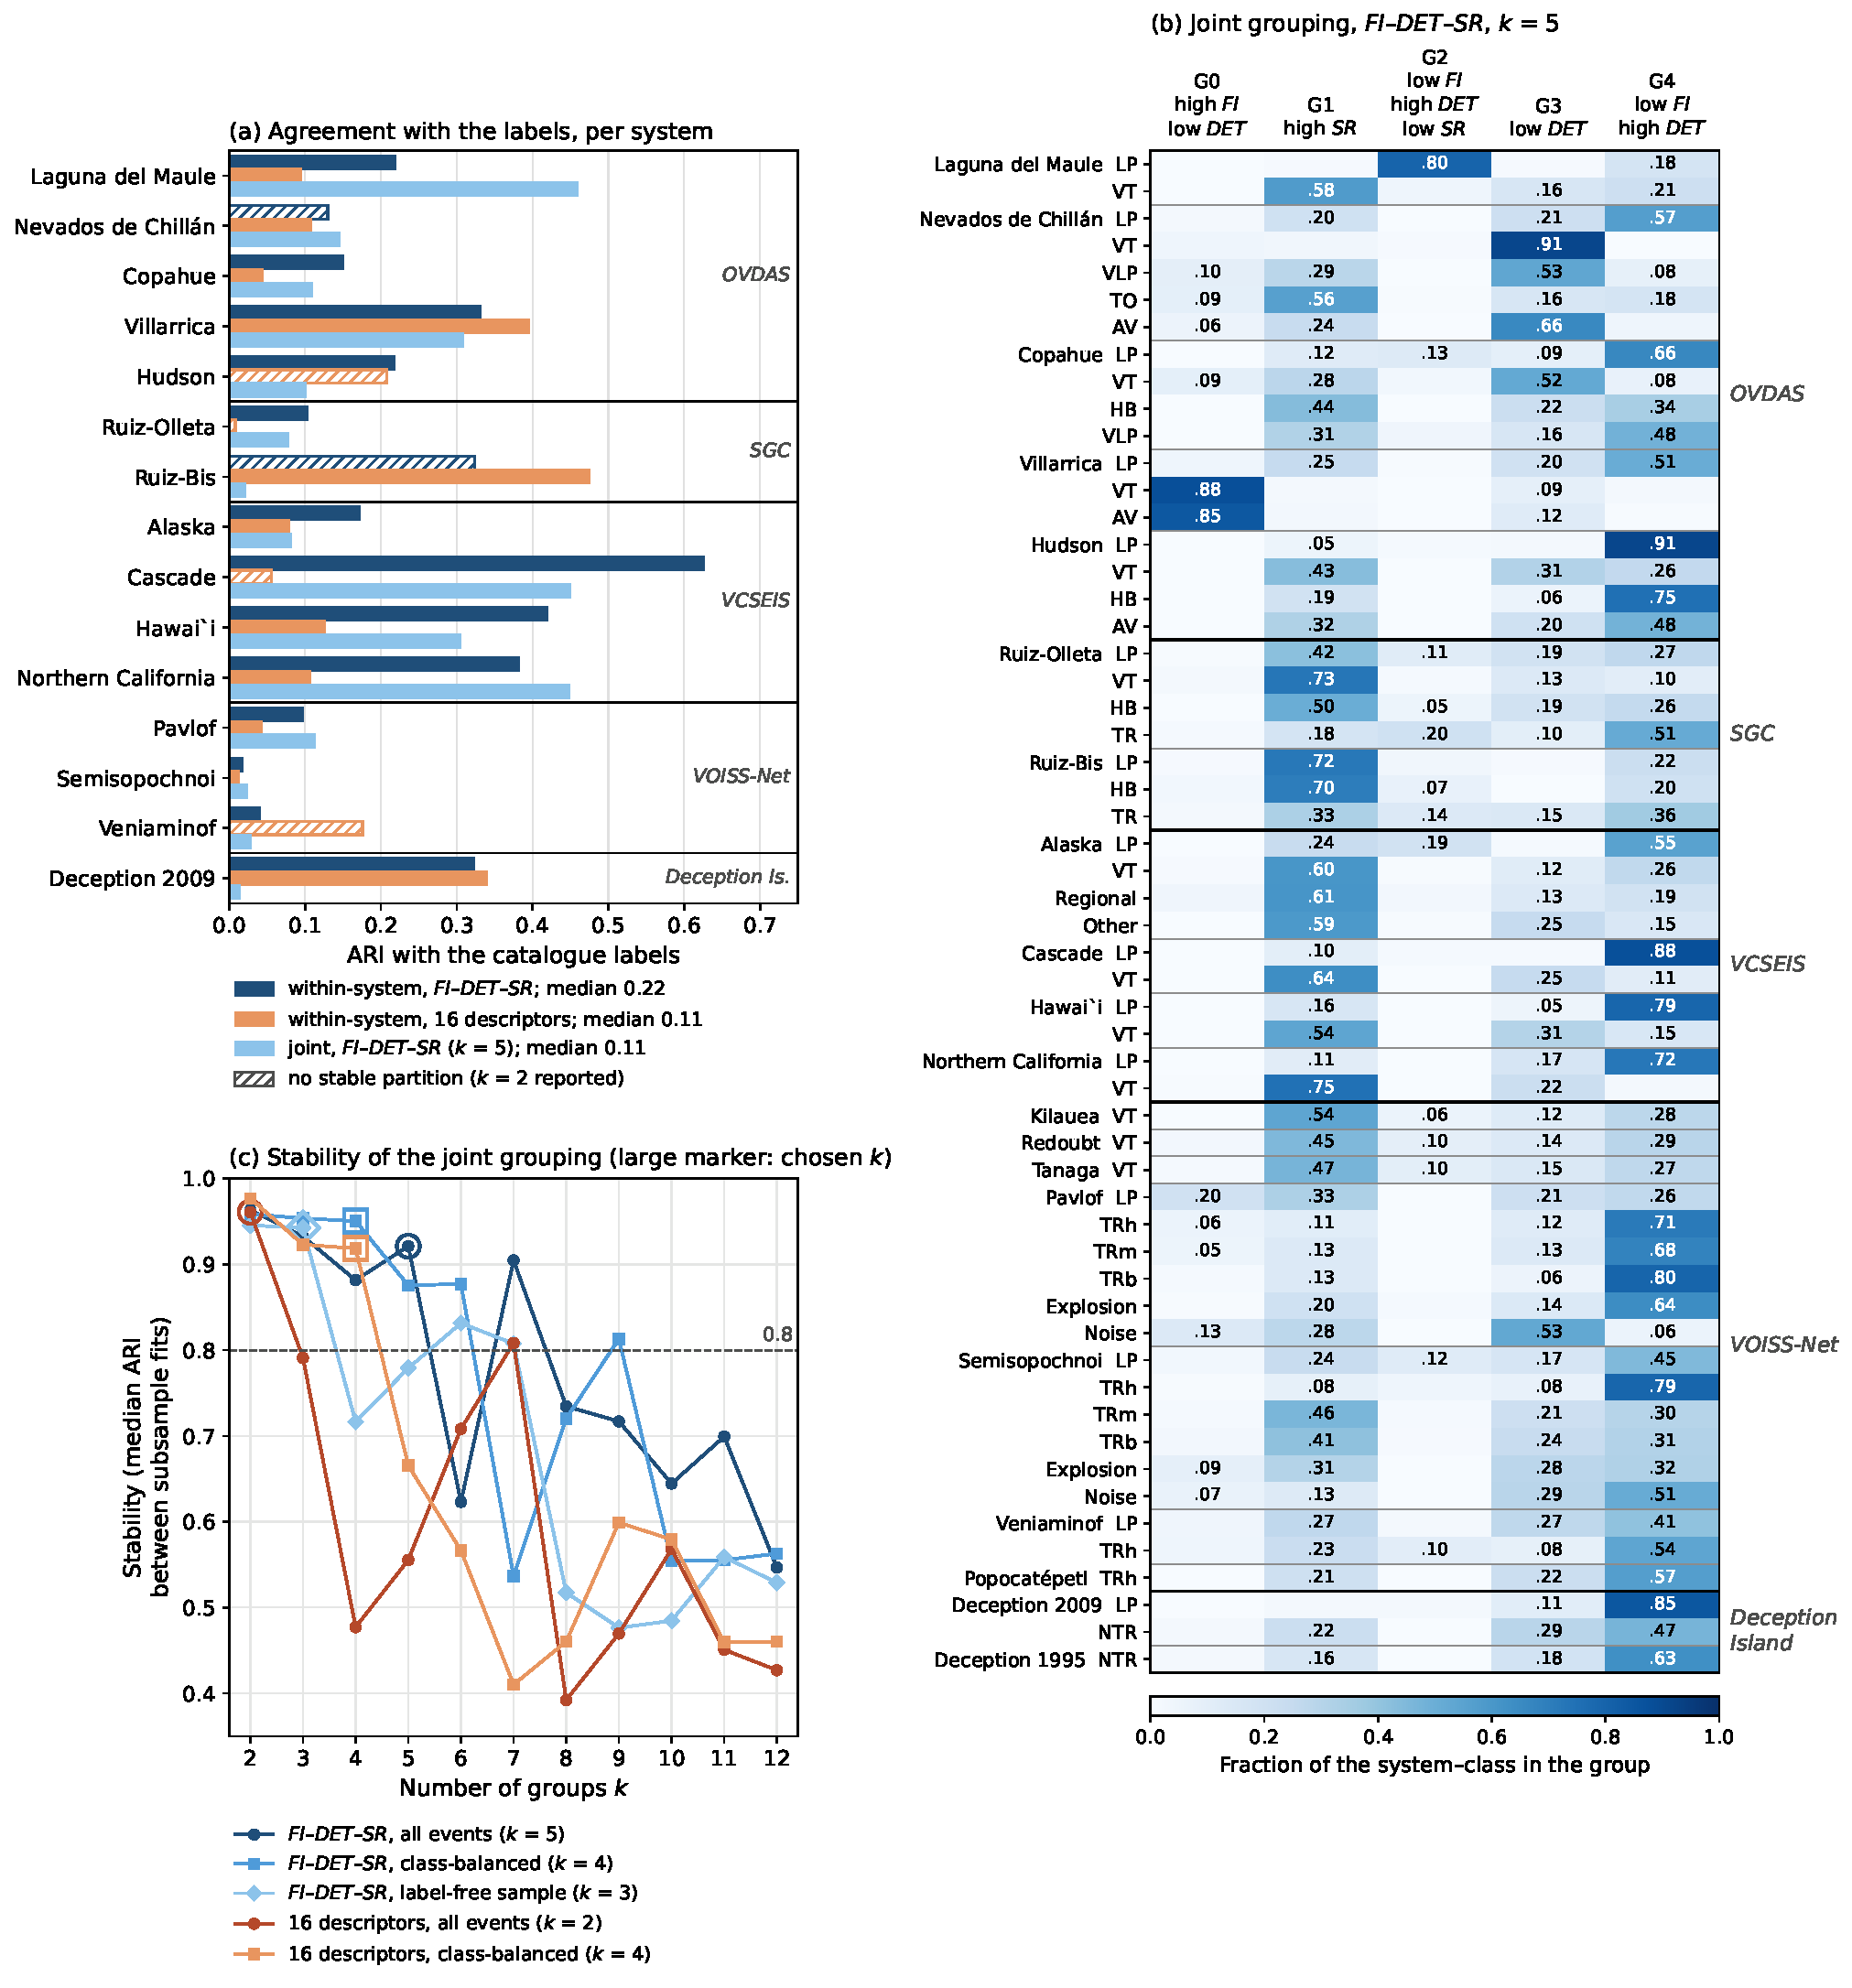
\includegraphics[width=0.98\textwidth]{fig_agrupamiento_paper.pdf}
\caption{Unsupervised grouping with Gaussian mixtures on the fixed-length
window. (a) Adjusted Rand index (ARI) between the groups and the catalog
labels at each system, for the grouping within each system on $FI$, $DET$
and $SR$ and on the sixteen descriptors, and for the joint five-component
grouping on $FI$, $DET$ and $SR$; hatched bars mark partitions with no stable
number of components, reported with two; single-class systems are omitted.
(b) Share of each class of each system in each group, G0 to G4, of that joint
grouping, described by the median over systems of the per-system medians of
$FI$, $DET$ and $SR$. (c) Stability of the joint grouping, the median ARI
between fits on subsamples, against the number of components $k$ for the
five variants; the dashed line marks the 0.8 threshold and large markers the
retained number.}
\label{fig:grouping}
\end{figure}

\section{Conclusion}\label{sec:conclusion}

\backmatter

\bmhead{Supplementary information}

\bmhead{Acknowledgements}

We thank John Makario Londo\~no and the Servicio Geol\'ogico Colombiano,
through its Observatorio Vulcanol\'ogico y Sismol\'ogico de Manizales, for
the Nevado del Ruiz events and the guidance on its reference stations, and
David Fee (Alaska Volcano Observatory, University of Alaska Fairbanks) for the
VOISS-Net labels and their documentation. We thank the authors of the
Deception Island databases \cite{cortes_vsr_2018} and of VCSEIS
\cite{zhong_deep-learning-based_2024} for making them public, and the Alaska
Volcano Observatory, the Hawaiian Volcano Observatory, the Northern California
Earthquake Data Center and the Pacific Northwest Seismic Network for the
catalogs behind VCSEIS. Waveforms of the AV, HV and 7G networks were accessed
through the data services of the EarthScope Consortium. The catalog and
records of the five Southern Andes systems come from the Observatorio
Volcanol\'ogico de los Andes del Sur (OVDAS), Servicio Nacional de Geolog\'ia
y Miner\'ia (SERNAGEOMIN).

\section*{Declarations}
\begin{itemize}
\item Funding: Not applicable.
\item Conflict of interest/Competing interests: Not applicable.
\item Ethics approval and consent to participate: Not applicable.
\item Consent for publication: Not applicable.
\item Data availability: % TODO
\item Materials availability: Not applicable.
\item Code availability: % TODO
\item Author contribution: % TODO
\end{itemize}

\begin{appendices}

\section{Supplementary material}\label{secA1}

\begin{table}[h]
\caption{Validation events analyzed, by system and class, each event counted
once. A cell gives the events with a fixed-length window and, after the
slash, those with a coda-length window; tremor and noise of VOISS-Net, tremor
of Nevado del Ruiz and NTR of Deception Island carry the fixed-length window
alone, and their single count applies to it. Dashes mark classes the system
does not label.}\label{tab:valcounts}
\begin{tabular}{@{}>{\raggedright\arraybackslash}p{0.17\linewidth}
                >{\raggedleft\arraybackslash}p{0.09\linewidth}
                >{\raggedleft\arraybackslash}p{0.09\linewidth}
                >{\raggedright\arraybackslash}p{0.55\linewidth}@{}}
\toprule
System & LP & VT & Local classes \\
\midrule
\multicolumn{4}{@{}l}{\textit{Deception Island}} \\
1995            & 48/38   & 29/19   & NTR 87 \\
2009            & 175/170 & 24/24   & NTR 435 \\
\multicolumn{4}{@{}l}{\textit{VCSEIS}} \\
Alaska          & 459/459 & 416/416 & regional 163/162, other 357/340, tremor 2/2, avalanche 1/1 \\
Cascade Range   & 170/164 & 186/183 & -- \\
Hawai`i         & 398/397 & 352/352 & -- \\
N. California   & 327/327 & 361/361 & -- \\
\multicolumn{4}{@{}l}{\textit{VOISS-Net}} \\
K\={\i}lauea    & --      & 878/878 & -- \\
Redoubt         & --      & 961/961 & -- \\
Tanaga          & --      & 936/936 & -- \\
Veniaminof      & 833/833 & --      & harmonic tremor 422 \\
Semisopochnoi   & 715/715 & --      & explosion 299/299; tremor 717 (harmonic 133, monochromatic 84, broadband 500); noise 500 \\
Pavlof          & 61/61   & --      & explosion 145/145; tremor 1{,}436 (harmonic 436, monochromatic 500, broadband 500); noise 500 \\
Popocat\'epetl  & --      & --      & harmonic tremor 500 \\
\multicolumn{4}{@{}l}{\textit{SGC, Nevado del Ruiz}} \\
Olleta          & 176/147 & 216/173 & HB 389/359; tremor pulses 250 \\
Bis             & 173/143 & 5/3     & HB 70/64; continuous tremor 250 \\
\botrule
\end{tabular}
\end{table}

\begin{figure}[H]
\centering
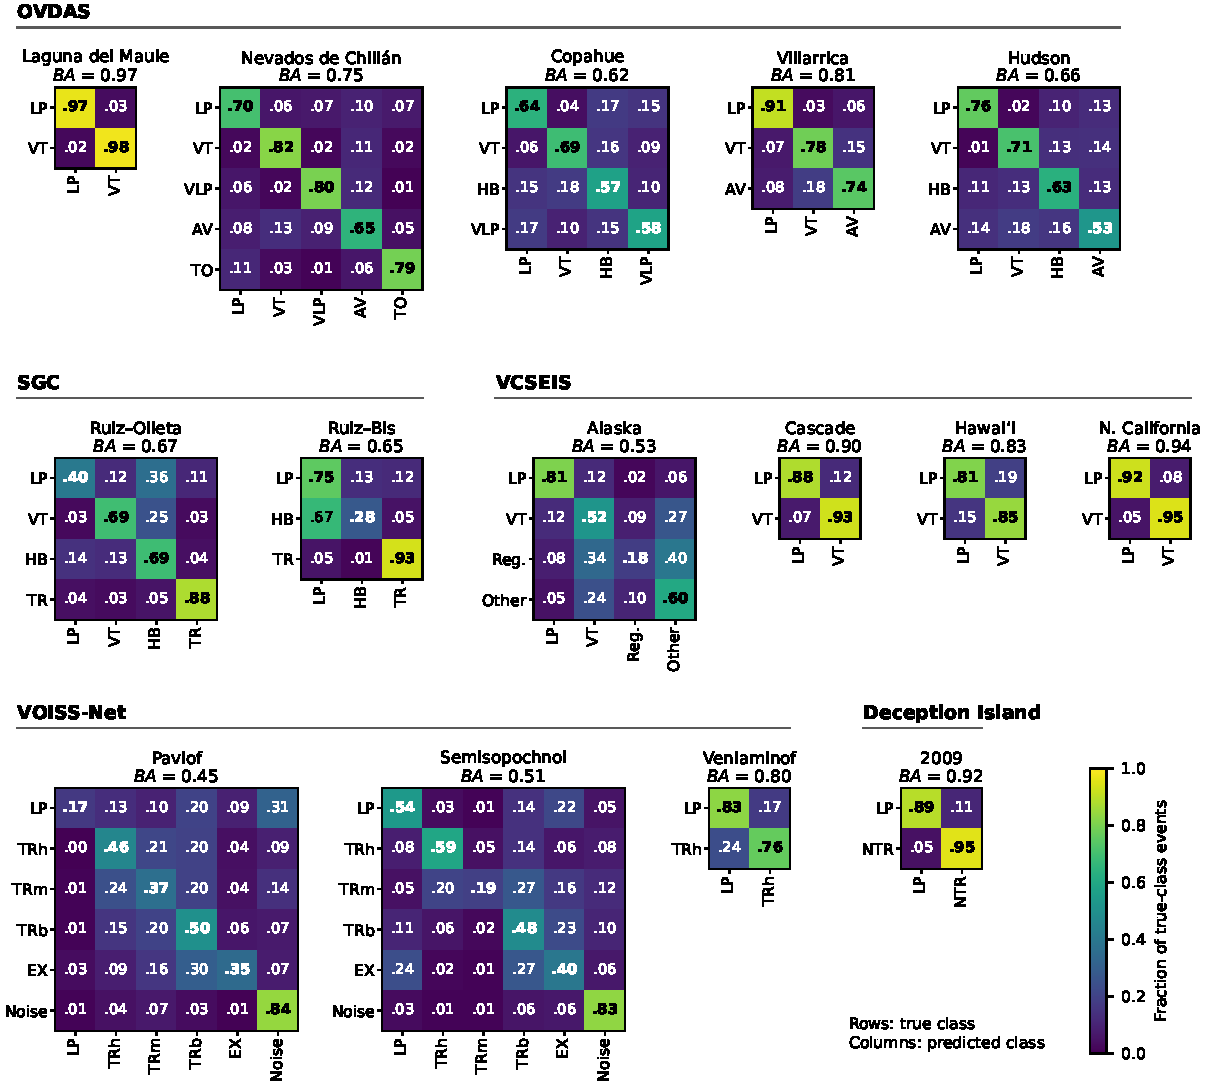
\includegraphics[width=0.98\textwidth]{fig_confusion_por_sistema.pdf}
\caption{Row-normalized confusion matrices of the multiclass classification
within each system (gradient-boosted trees, fixed-length window), accumulated
over five repetitions of five-fold cross-validation with every class of at
least 50 events. Rows give the true class and columns the predicted class, so
each off-diagonal entry is the fraction of a class taken for another and
measures their overlap. Panels are grouped by agency or catalog, and each
title gives the system and its balanced accuracy (BA); Ruiz--Olleta and
Ruiz--Bis are Nevado del Ruiz at Olleta and at Bis. Reg.: regional events;
TRh, TRm, TRb: harmonic, monochromatic and broadband tremor; EX: explosions;
NTR: noise and tremor class of Deception Island.}
\label{fig:confusion}
\end{figure}

\begin{figure}[H]
\centering
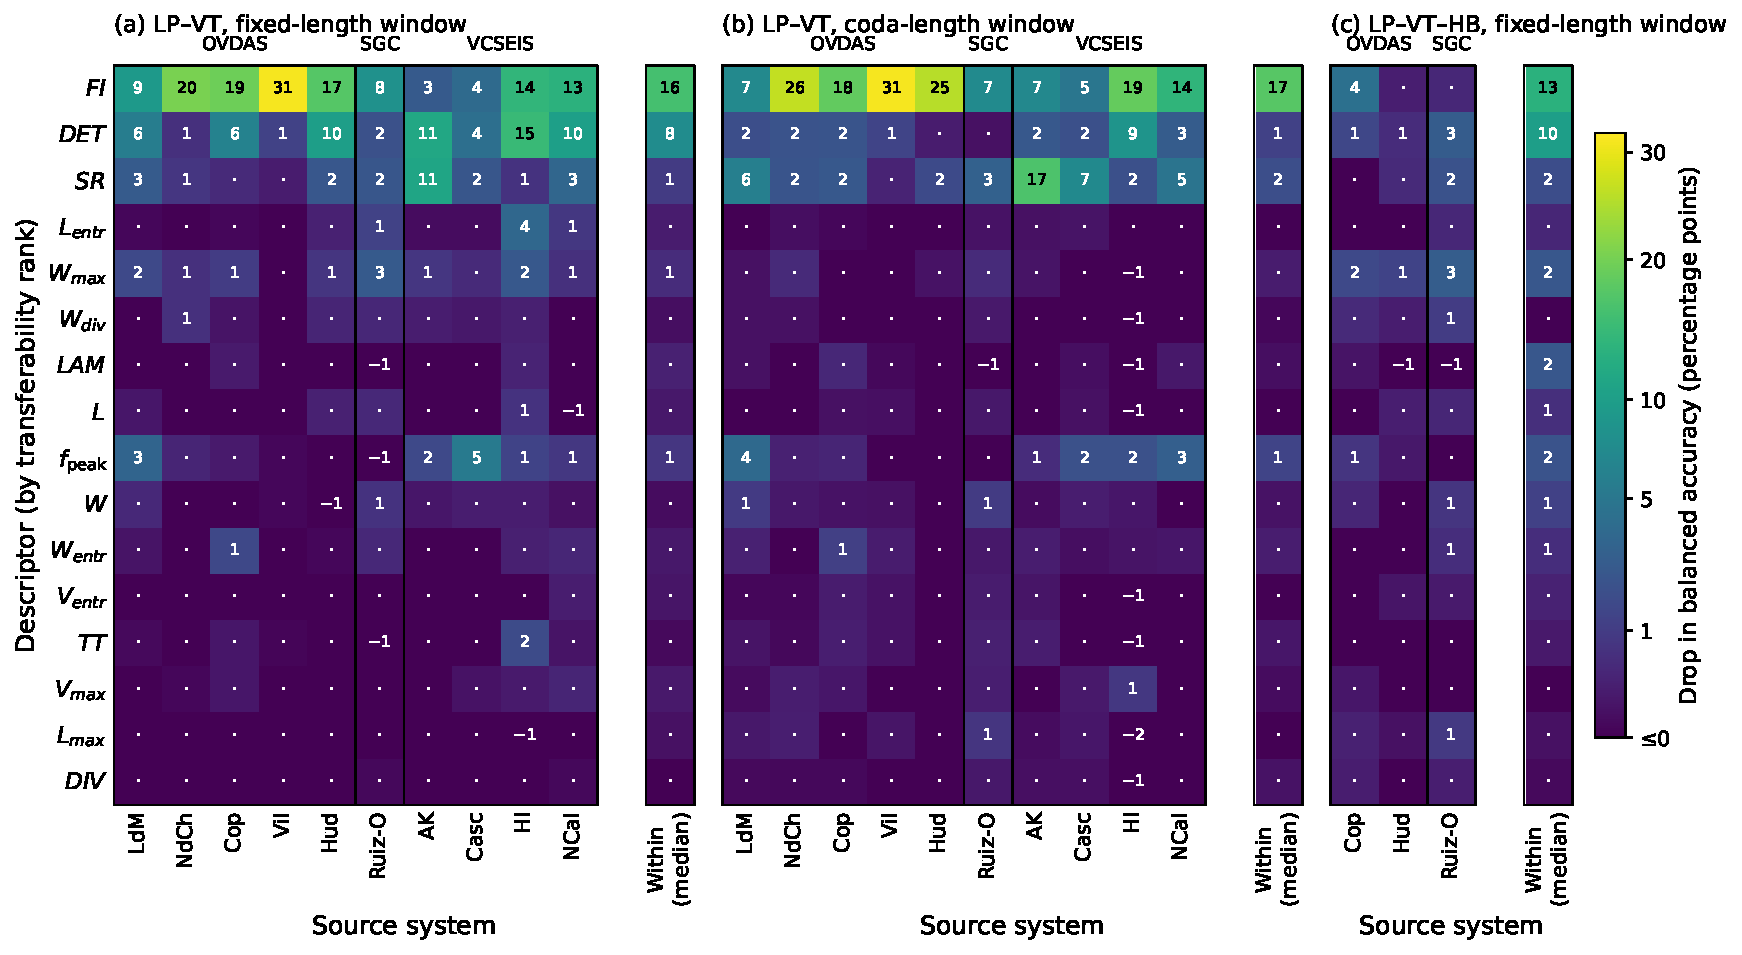
\includegraphics[width=0.98\textwidth]{fig_importancia.pdf}
\caption{Permutation importance of the sixteen descriptors in transfer
between systems (gradient-boosted trees, source scaling): (a) LP--VT,
fixed-length window; (b) LP--VT, coda-length window; (c) LP--VT--HB,
fixed-length window. Each cell gives the median, over the targets other than
the source, of the drop in balanced accuracy in percentage points when the
descriptor is permuted (mean of three training draws); dots mark values within
half a point of zero. Columns are source systems grouped by agency, abbreviated as in
Figure~\ref{fig:matrices}; the separate column gives the median
within-system importance, and rows follow the fixed-window transferability
ranking.}
\label{fig:importance}
\end{figure}

\end{appendices}

\bibliography{references}

\end{document}